\chapter{Entangling unravellings for quantum state engineering / Results}

The central question of this chapter is whether independent local dissipative channels can be turned into a resource for conditional entanglement generation. At the unconditional level, the answer is clearly negative as long as the two environmental outputs are treated locally. Indeed, if the reduced dynamics is described by two independent channels acting on the two qubits, the corresponding dynamical map factorizes as
\begin{equation}
	\Phi_t = \Phi_t^{(1)} \otimes \Phi_t^{(2)}.
	\label{eq:chapter3_local_channel_factorization}
\end{equation}
For an arbitrary separable initial state
\begin{equation}
	\rho_{\mathrm{sep}}(0)
	=
	\sum_j p_j\,\rho_j^{(1)} \otimes \rho_j^{(2)},
	\qquad
	p_j \geq 0,
	\qquad
	\sum_j p_j = 1,
	\label{eq:chapter3_generic_separable_state}
\end{equation}
one then has
\begin{equation}
	\rho_{\mathrm{sep}}(t)
	=
	(\Phi_t^{(1)} \otimes \Phi_t^{(2)})\rho_{\mathrm{sep}}(0)
	=
	\sum_j p_j\,\Phi_t^{(1)}[\rho_j^{(1)}]\otimes \Phi_t^{(2)}[\rho_j^{(2)}],
	\label{eq:chapter3_local_maps_preserve_separability}
\end{equation}
which is still a convex combination of product states. Therefore, local channels preserve separability and cannot generate entanglement from initially separable states.

This observation identifies the only possible route toward a non-trivial conditional dynamics: the information leaking into the environment must be processed in a nonlocal way before detection. 
With this motivation in mind, we first review the fluorescence-based scheme, which provides the clearest illustration of the general mechanism. We then move to the setup studied in this thesis, where the same interferometric logic is applied to two independent local dephasing channels.

\section{Measurement-induced entanglement in the fluorescence scheme}
\label{sec:lewalle_fluorescence_review}

Before introducing our dephasing-based setup, it is useful to briefly review the fluorescence scheme discussed by Lewalle \textit{et al.} in Ref.~\cite{Lewalle21}. Even though the microscopic dissipation mechanism is different, the operational logic is very close to the one employed in this thesis. In both cases, the key idea is to start from two independent local channels, interfere the corresponding output modes on a beam splitter, and then monitor suitable combinations of them. Entanglement is not generated by a direct interaction between the two qubits, but by the measurement backaction associated with a joint detection scheme.

\begin{figure}[h!]
	\centering
	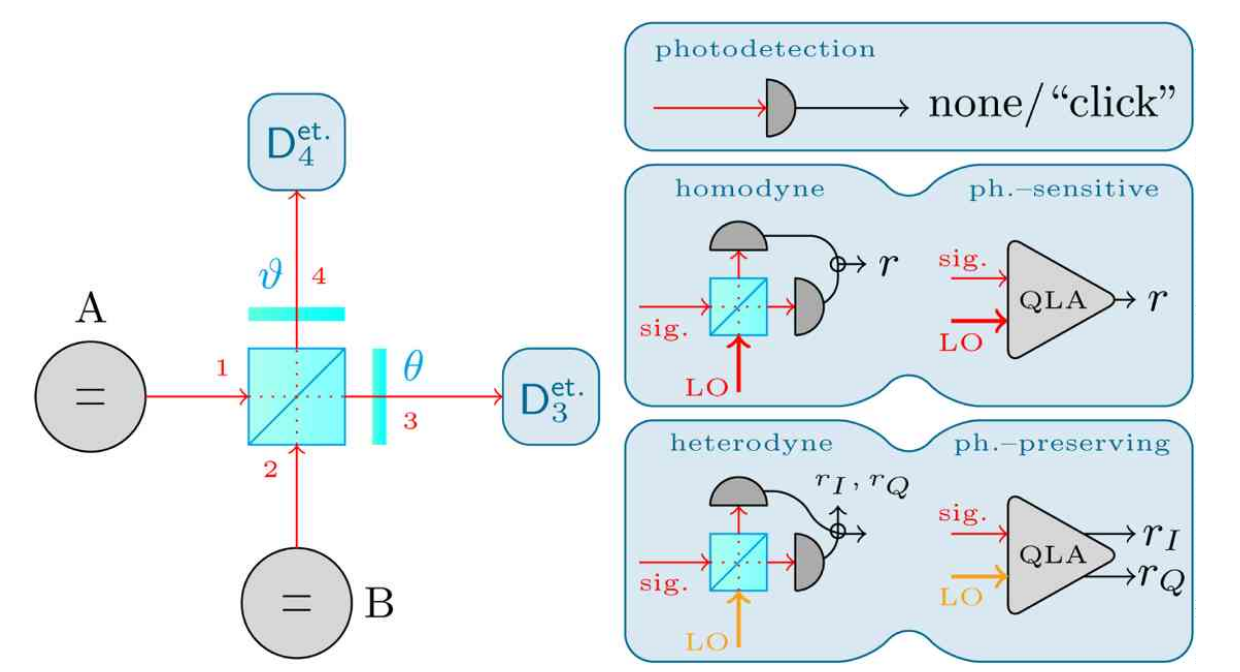
\includegraphics[width=0.8\textwidth]{Images/Cap3/Setup_Jordan.png}
	\caption{Schematic representation of the measurement setup. Two remote qubits emit into two independent output modes, which are mixed on a balanced beam splitter and then monitored at the two output ports. The relative phases in the two paths are controlled by phase shifters. Different choices of detection at the output, namely photodetection, homodyne, or heterodyne measurement, correspond to different unravellings of the same open-system dynamics. Adapted from Ref.~\cite{Lewalle21}.}
	\label{figure_Setup_Jordan}
\end{figure}

The physical scenario considered in the review consists of two distant and non-interacting quantum emitters, each coupled to its own radiative environment. The emitted fluorescence from the two sites is collected and sent to a common optical stage. The central optical element is a balanced beam splitter, which mixes the two outgoing modes before they are measured. Additional phase plates can be placed after the beam splitter, so that the fields arriving at the two output ports acquire controllable phases. The final detection stage is implemented at the two output ports, labeled \(3\) and \(4\), either by photon counters or by quadrature measurements. In this way one does not monitor the two local emissions separately but rather monitors their interferometrically mixed combinations. We notice that this device geometry is closely related to the one commonly employed for Bell-state measurements. It follows that a crucial feature is that it allows the creation of entanglement between distant qubits without any direct qubit-qubit coupling: the only resource is the information extracted from the optical measurement. In other words, coherent correlations are established entirely through the inferences that can be drawn from the joint monitoring of the emitted light. From this point of view, the setup realizes a measurement-induced entangling mechanism.

In this setup reviewed by Lewalle, to each qubit is associated a spontaneous-emission operator, $\hat{\sigma}^{(A)}_-$ and $\hat{\sigma}^{(B)}_-$. After the balanced beam splitter and the phase shifters, the measured optical modes correspond to linear combinations of the two original fluorescence outputs. The relevant thing is that once the two fields have been mixed, a detector click or a homodyne current at one output port generally cannot be attributed to one emitter alone. The detection event is associated with a coherent superposition of the two local decay paths.

This is the origin of the connection with which-path information. If the measurement reveals which emitter produced the signal, then the two decay paths remain distinguishable and no entanglement is created. If, on the contrary, the optical mixing and the chosen measured quadratures erase that information, then the backaction acts jointly on the two-qubit state and may generate entanglement. In the review, this mechanism is repeatedly interpreted in terms of information erasure and, more conceptually, as a continuous-variable version of entanglement swapping. This viewpoint is especially natural in the optimal homodyne configuration, where the joint measurement performed on the output fields can be regarded as a continuous-variable EPR-basis measurement. At the intermediate stage of the dynamics, one has two bipartite correlations: qubit \(A\) is correlated with mode \(1\), and qubit \(B\) is correlated with mode \(2\) but the optical measurement performed after the beam splitter does not probe these two modes independently. Instead, it performs a joint measurement on the mixed output modes. The role of this measurement is then to convert the initial qubit-field correlations into qubit-qubit correlations.
The continuous-variable character of this mechanism is encoded in the observables
\begin{equation}
	\hat X_+ = \hat X_1 + \hat X_2,
	\qquad
	\hat P_- = \hat P_1 - \hat P_2.
	\label{eq:cv_epr_observables}
\end{equation}
These two operators commute and therefore can be measured jointly. Their simultaneous measurement defines an EPR-type basis for the two optical modes. If the corresponding readouts are denoted by \(r_+\) and \(r_-\), the measurement projects the fields onto a state characterized by the relations $X_1 + X_2 = r_+$ and $P_1 - P_2 = r_-$. In the idealized case \(r_+=0\) and \(r_-=0\), one obtains the maximally correlated EPR condition: the two field quadratures are perfectly anticorrelated in position and perfectly correlated in momentum \cite{Braunstein98}.

From this perspective, the role of which-path information becomes especially clear. If the measurement preserves enough information to distinguish whether the signal originated from emitter \(A\) or emitter \(B\), then the optical projection remains effectively local or separable, and no entanglement swap can occur. By contrast, if the measurement erases the path information, then the optical modes are projected onto an entangled basis, and the qubit-mode correlations can be transferred to the qubits themselves.

In optimal homodyne configuration the measured quadratures correspond to a joint measurement of nonlocal combinations of the two optical modes, the measurement basis is therefore entangled and the two-qubit are conditioned by an entanglement-swapping mechanism.

%The opposite situation occurs when the chosen quadratures maximize path distinguishability. In that regime, the optical measurement can be re-expressed as a measurement of local observables on modes \(1\) and \(2\). The corresponding optical post-measurement state is then separable, not EPR-like, and no entanglement can be transferred to the two qubits. In this sense, which-path information erasure and entanglement swapping are not two independent explanations of the same phenomenon. They are two complementary descriptions of a single mechanism. Erasing the path information means projecting the optical subsystem onto an entangled measurement basis, and this is exactly what allows the entanglement initially shared between each qubit and its local field to be swapped into entanglement between the two remote qubits.

%This interpretation is conceptually useful also for the results discussed later. It explains why the optimal measurement does not create entanglement from nothing. The relevant resource is already present in the qubit-field correlations generated by the emission process. The measurement only redistributes that resource. When the optical readout is chosen in a way that preserves indistinguishability, the redistribution is optimal. When part of the path information is retained, part of that resource is wasted, and the attainable two-qubit entanglement is correspondingly reduced.

\subsection{Analyzing photodetection}

We start by reviewing the photodetection measurement setup. In that case one counts photons at the two output ports \(3\) and \(4\). If both qubits are initially prepared in the excited state $\ket{e}=\ket{0}$, the first detected photon projects the two-qubit state into the single-excitation sector. Because the two fluorescence channels have already been interferometrically mixed, this first detection event does not identify which qubit decayed. Instead, it prepares one of the entangled Bell-like states in the odd sector. The second detected photon then completes the relaxation towards the ground state $\ket{g}=\ket{1}$.

This result follows from the structure of the individual quantum trajectories. Starting from \(\ket{ee}\), there are only three relevant possibilities at time \(t\): no emission has occurred, exactly one emission has occurred, or two emissions have occurred. In the ideal photodetection scheme, these three cases correspond to three qualitatively different conditional states. If no photon has been detected up to time \(t\), the two-qubit state remains in the fully excited separable state \(\ket{ee}\), and its concurrence is therefore zero. If exactly one photon has been detected, the detection event projects the system onto the single-excitation Bell sector, so that the conditional state is maximally entangled and its concurrence is equal to one. Finally, if two photons have been detected, both qubits have decayed and the system is in the separable ground state \(\ket{gg}\), whose concurrence is again zero.

Hence, for each trajectory, the concurrence takes only the values
\begin{equation}
	C(t)=
	\begin{cases}
		0, & \text{no click up to } t,\\
		1, & \text{exactly one click up to } t,\\
		0, & \text{two click up to } t.
	\end{cases}
\end{equation}
The trajectory-averaged concurrence is then simply $\overline{C}(t)=\mathbb{E}[C(t)]=P_1(t)$ where \(P_1(t)\) is the probability that exactly one decay has occurred by time \(t\).

Since the two emitters decay independently with rate \(\gamma\), the probability that one given emitter is still excited at time \(t\) is \(e^{-\gamma t}\), while the probability that it has already decayed is \(1-e^{-\gamma t}\). Therefore, the probability that exactly one decay has occurred is obtained by summing the two mutually exclusive possibilities: emitter \(A\) decays while emitter \(B\) does not, or emitter \(B\) decays while emitter \(A\) does not. This gives
\begin{equation}
	\overline{C}(t) = P_1(t)
	=
	e^{-\gamma t}\left(1-e^{-\gamma t}\right)
	+
	e^{-\gamma t}\left(1-e^{-\gamma t}\right)
	=
	2e^{-\gamma t}\left(1-e^{-\gamma t}\right).
	\label{eq:lewalle_photodetection_avg_concurrence} 
\end{equation}

\begin{figure}[h!]
	\centering
	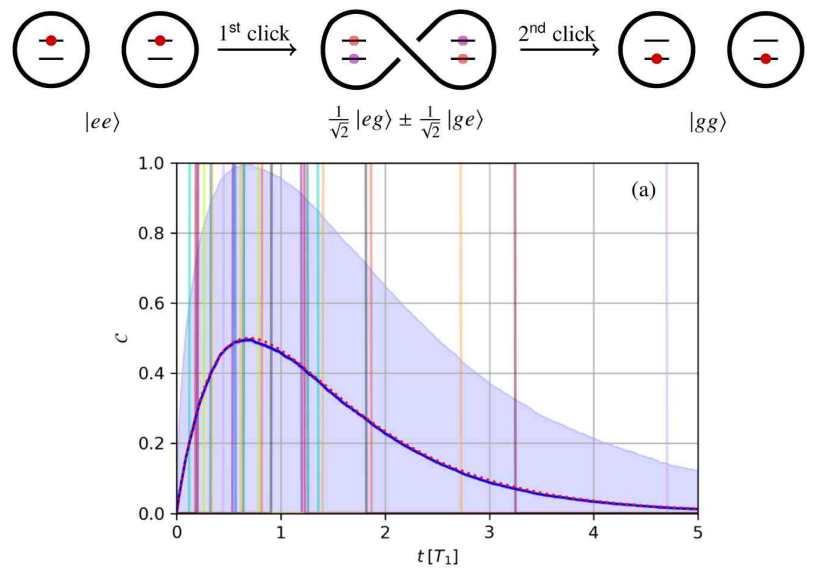
\includegraphics[width=0.8\textwidth]{Images/Cap3/Jordan_phdet_++.png}
	\caption{Ideal photodetection dynamics for two emitters initially prepared in \(\ket{ee}\). In the lower panel, the horizontal axis reports the rescaled time \(t/T_1\), while the vertical axis shows the concurrence \(C\). The solid curve represents the trajectory-averaged concurrence, as given by Eq.~\eqref{eq:lewalle_photodetection_avg_concurrence}, whereas the vertical colored lines denote the click times for different individual trajectories. The upper panel illustrates the corresponding jump mechanism.}
	\label{figure_photodetection_Jordan}
\end{figure}

As we can see $\overline{C}(t)$ vanishes at \(t=0\), reaches its maximum at intermediate times, and then decays back to zero as both emitters relax to the ground state. The result is particularly transparent: the concurrence tracks the probability that one, but not both, emission events has occurred.

\subsection{Optimal homodyne phases}

A different situation arises when the two output ports are monitored by homodyne detection. In this case the measurement record is continuous, and the conditional state follows diffusive stochastic trajectories. Starting from \(\ket{ee}\), the system evolves continuously toward \(\ket{gg}\), and entanglement is generated gradually rather than through isolated jumps.

The relevant ingredient is now the choice of the local-oscillator phases. Since the two beam-splitter outputs are measured in selected quadratures, the relative phases determine whether the measurement preserves or erases which-path information. Analogously as before, if the chosen quadratures still allow one to distinguish which qubit contributed to the signal, entanglement generation is suppressed.

The optimal condition is when
\begin{equation}
	|\theta-\vartheta|=\frac{\pi}{2},
\end{equation}
for example
\begin{equation}
	\theta=0,
	\qquad
	\vartheta=\frac{\pi}{2}.
\end{equation}
In this configuration the two homodyne detectors measure quadratures that differ by \(90^\circ\). This is precisely the condition under which the two local decay paths become indistinguishable at the level of the measurement record.

\ref{figure_homodyne_Jordan} summarizes the consequences of this choice. In the left panel, one sees the average concurrence together with several individual trajectories, all starting from \(\ket{ee}\). For the optimal phases, many trajectories rise well above the average value, and some reach \(C=1\). Unlike photodetection, however, this occurs through a smooth diffusive evolution rather than through abrupt jumps.

\begin{figure}[h!]
	\centering
	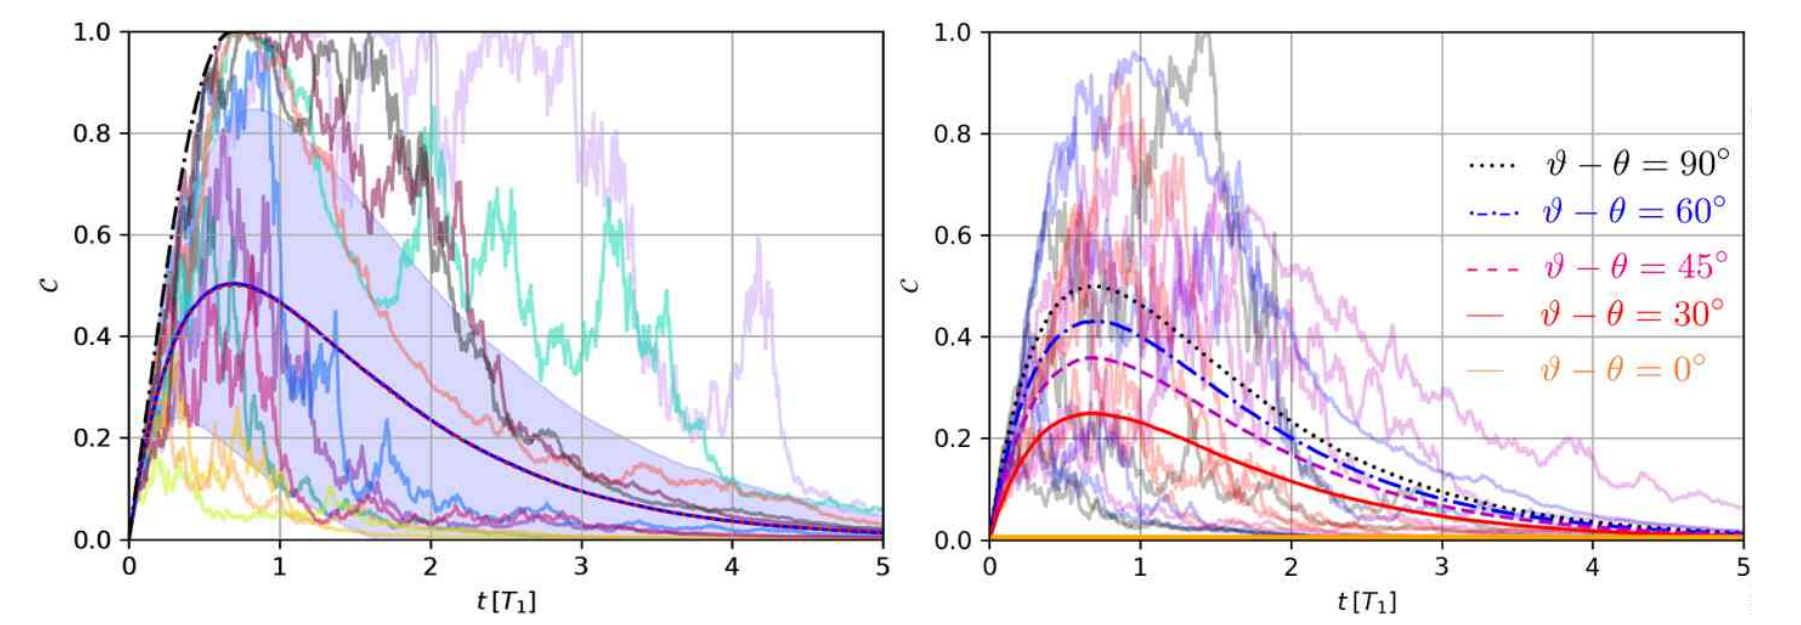
\includegraphics[width=0.8\textwidth]{Images/Cap3/Jordan_hom_++.png}
	\caption{Homodyne entanglement generation starting from \(\ket{ee}\). In both panels, the horizontal axis reports the rescaled time \(t/T_1\), while the vertical axis shows the concurrence \(C\). Left panel: individual diffusive trajectories and corresponding trajectory-averaged concurrence for the optimal homodyne phases. Right panel: average concurrence for different relative phase differences \(\vartheta-\theta\). The maximal entanglement yield is obtained for \(|\vartheta-\theta|=\pi/2\), while deviations from this condition reduce the concurrence by progressively restoring which-path distinguishability.}
	\label{figure_homodyne_Jordan}
\end{figure}


Although the individual trajectories are qualitatively different, the optimal homodyne scheme yields the same concurrence as ideal photodetection \eqref{eq:lewalle_photodetection_avg_concurrence},
\begin{equation}
	\overline{C}(t)
	=
	2e^{-\gamma t}\left(1-e^{-\gamma t}\right).
	\label{eq:lewalle_homodyne_avg_concurrence}
\end{equation}

\subsection{Measurement inefficiency and physical implications}

A relevant non-ideal extension is obtained by considering inefficient detection. Operationally, this is modeled by inserting additional unbalanced beam splitters after the main \(50/50\) beam splitter, so that only a fraction \(\eta\in[0,1]\) of the fluorescence reaches the detectors, while the remaining fraction \(1-\eta\) is lost. Inefficiency makes part of the emitted information inaccessible and as a consequence, the conditional state is no longer pure, because the observer must average over undetected emission events.

This has a direct physical meaning: after a no-click interval, one cannot conclude that no photon has been emitted. One can only conclude that no photon has been detected. A missed emission is always possible, and this uncertainty degrades the observer's knowledge of the two-qubit state. In particular, a detected click can no longer be interpreted with certainty as the first emission event.

In the photodetection case, this loss of information has two main consequences. First, the average concurrence retains the same qualitative time dependence as in the ideal case, but with a reduced overall amplitude:
\begin{equation}
	\overline{C_{\eta}(t)}
	\approx
	2\eta\,e^{-\gamma t}\left(1-e^{-\gamma t}\right).
	\label{eq:lewalle_ineff_avg_concurrence}
\end{equation}
Thus, inefficiency lowers the average entanglement yield without changing the basic temporal profile.

Second, the concurrence attainable in a single realization is no longer allowed to reach unity at arbitrary times. In the ideal case, a detected click can project the system onto a Bell state. For \(\eta<1\), this is no longer guaranteed, because one or more previous photons may have been emitted and lost. The conditional state after a detected click is then a mixture of an entangled contribution and a separable one and it causes that the maximal concurrence decreases with time.

The detected click is therefore no longer a reliable witness that the system have just entered the single-excitation sector. This is precisely why the attainable concurrence is reduced.

These observations are directly relevant for the present work. They show that interferometric mixing alone is not sufficient to guarantee efficient measurement-induced entanglement generation. The protocol also requires that a sufficiently large fraction of the emitted information be actually collected. More generally, the tutorial makes clear that the entangling power of the monitoring scheme is controlled by two ingredients: the measurement basis, which determines whether which-path information is erased or preserved, and the detection efficiency, which determines how much of that information remains available to the observer.


\begin{comment}
\section{Convention, states and master equation}

We consider a system of $N=2$ qubits, each described in the computational basis
$\{\ket{0},\ket{1}\}$.
Throughout this work we adopt the convention
\begin{equation}
	\sigma_z \ket{1} = + \ket{1}, 
	\qquad
	\sigma_z \ket{0} = - \ket{0},
\end{equation}
so that the excited state $\ket{1}$ corresponds to the positive eigenvalue of $\sigma_z$.
This choice fixes all relative signs in the collective spin operators and in the dissipative dynamics.

The single-qubit spin operators are defined as
\begin{equation}
	S_\alpha^{(i)} = \frac{1}{2}\,\sigma_\alpha^{(i)},
	\qquad \alpha \in \{x,y,z\},
\end{equation}
where the superscript $i$ labels the qubit.
Collective spin operators are introduced as
\begin{equation}
	J_\alpha = \sum_{i=1}^{N} S_\alpha^{(i)}.
\end{equation}

When needed, spin coherent states (CSS) are written as
\begin{equation}
	\ket{\theta,\phi}_{N}
	=
	\bigotimes_{i=1}^{N}
	\left(
	e^{i\phi}\sin\frac{\theta}{2}\,\ket{1}_i
	+
	\cos\frac{\theta}{2}\,\ket{0}_i
	\right),
	\label{CSS_N_qubit}
\end{equation}
which corresponds to a product state with all spins pointing along the direction
$\hat{n} = (\sin\theta\cos\phi,\sin\theta\sin\phi,\cos\theta)$ on the Bloch sphere.
We explicit the case for N=2 and $\phi=0$:
\begin{equation}
	\ket{\theta} \equiv \ket{\theta,0}_{2}
	=\sin^2\frac{\theta}{2}\ket{11}
	+\sin\frac{\theta}{2}\cos\frac{\theta}{2}\left(\ket{10}+\ket{01}\right)
	+\cos^2\frac{\theta}{2}\ket{00}.
	\label{CSS_expansion_2}
\end{equation}
In particular, the eigenstates of $\sigma_x$ are
\begin{equation}
	\ket{+}=\frac{\ket{0}+\ket{1}}{\sqrt{2}},
	\qquad
	\ket{-}=\frac{\ket{0}-\ket{1}}{\sqrt{2}}.
\end{equation}

	We use the standard Bell states
\begin{align}
	\ket{\phi_\pm}&=\frac{\ket{00}\pm\ket{11}}{\sqrt{2}}
	\quad(\text{even $z$-parity}),\\
	\ket{\psi_\pm}&=\frac{\ket{01}\pm\ket{10}}{\sqrt{2}}
	\quad(\text{odd $z$-parity}).
\end{align}

The dynamics of the system is described within the Markovian open-quantum-system framework.
Under the standard assumptions of weak system-environment coupling, short bath correlation time
(Born-Markov approximation), and complete positivity, the reduced density operator $\rho(t)$
obeys a Gorini--Kossakowski--Sudarshan--Lindblad (GKSL) master equation,
\begin{equation}
	\frac{d\rho}{dt} = \liouvillian_{k} [\rho_t]
	= - i \left[ H, \rho^{(c)} \right] + \sum_k \mathcal{D}[C_k]\rho^{(c)}\,dt = 
	- i \left[ H, \rho \right]
	+
	\sum_k
	\left(
	C_k \rho C_k^\dagger
	-
	\frac{1}{2}
	\left\{
	C_k^\dagger C_k,\rho
	\right\}
	\right).
	\label{eq:Lindblad}
\end{equation}
where $\mathcal{D}[A]\rho = A\rho A^\dagger - \tfrac{1}{2}\{A^\dagger A,\rho\}$ is called the dissipator superoperator. Here $H$ is the system Hamiltonian,
and $\{C_k\}$ are the Lindblad or collapse operators describing dissipative processes and continuous measurements.
We remark that equation~\eqref{eq:Lindblad} generates a completely positive and trace-preserving (CPTP) dynamical semigroup.

%Aggiunta nuovo paper Albarelli-Genoni-Rossi
In this work we focus on dissipative channels associated with spin components along the $z$ direction that acts independently on each qubit with strength $\gamma$. We can therefore write the master equation as:

\begin{equation}
	\frac{d\rho_t}{dt}
	= - i \left[ H, \rho_t \right] + \sum_{k=1}^{2} \mathcal{D}[\sigma_z^{(k)}]\rho^{(c)}_t\,dt
\label{ME_sigma_z}
\end{equation}

By exploiting $\sigma_z^{\dagger}=\sigma_z$ and $\sigma_z^{2}=\id$ we can rewrite $\eqref{ME_sigma_z}$ as:

\begin{equation}
	\frac{d\rho_t}{dt} = \liouvillian_{\gamma}
	= -i \dfrac{\omega}{2} \sum_{k=1}^{2}[\sigma_z^{(k)}, \rho_t] + \dfrac{\gamma}{2} (\sum_{k=1}^{2}\sigma_z^{(k)}\rho_t \sigma_z^{(k)} -N\rho_t)
	\label{ME_simplified}
\end{equation}

A central role is played by collective jump operators of the form:
\begin{equation}
	\hat{C}_\pm
	=
	\sqrt{\gamma}\,
	\frac{\sigma_z^{(1)} \pm \sigma_z^{(2)}}{\sqrt{2}}
	\label{eq:Lindblad_operators}
\end{equation}

These operators naturally arise in measurement schemes where emissions from the two qubits are interfered
(e.g.\ via a beam splitter) before detection, such that the measurement does not reveal which-path information.
The two channels correspond to symmetric and antisymmetric combinations of local $z$-spin operators.
While the master equation~\eqref{eq:Lindblad} uniquely determines the evolution of the density operator,
its stochastic unravelling into quantum trajectories is not unique (see Appendix A).
Different measurement schemes (photodetection, homodyne, heterodyne) correspond to different
stochastic evolutions at the level of pure states, all reproducing the same ensemble-averaged dynamics.

In the photodetection unravelling associated with the jump operators~\eqref{eq:Lindblad_operators},
the system undergoes non-unitary no-click evolution interrupted by quantum jumps.
Each jump corresponds to the application of $\hat{C_\pm}$ to the state vector,
followed by normalization, and reveals information about collective spin observables and parity.

This measurement backaction is the key mechanism exploited in this work for the generation
and stabilization of entanglement and for the study of quantities such as
concurrence and spin squeezing.

\section{Unitary invariance of Lindblad operators}

Let $U$ be an $n\times n$ unitary matrix acting on the vector of collapse operators $\{\hat C_i\}$.
We prove the identity
\begin{equation}
	\sum_{i=1}^{n}\mathcal{D}[\hat C_i]\rho
	=
	\sum_{i=1}^{n}\mathcal{D}\!\left[\sum_{j=1}^{n}U_{ij}\hat C_j\right]\rho,
	\label{eq:unitary_invariance_dissipator}
\end{equation}
where $\mathcal{D}[A]\rho=A\rho A^\dagger-\tfrac{1}{2}\{A^\dagger A,\rho\}$.

We expand the right-hand side:
\begin{align}
	\sum_i \mathcal{D}\!\left[\sum_j U_{ij}\hat C_j\right]\rho
	&=
	\sum_i
	\left[
	\left(\sum_j U_{ij}\hat C_j\right)\rho
	\left(\sum_k U_{ik}\hat C_k\right)^\dagger
	-
	\frac{1}{2}
	\left\{
	\left(\sum_j U_{ij}\hat C_j\right)^\dagger
	\left(\sum_k U_{ik}\hat C_k\right),
	\rho
	\right\}
	\right]\nonumber\\
	&=
	\sum_i
	\left[
	\sum_{j,k}U_{ij}U_{ik}^*\,\hat C_j\rho \hat C_k^\dagger
	-
	\frac{1}{2}
	\left\{
	\sum_{j,k}U_{ij}^*U_{ik}\,\hat C_j^\dagger \hat C_k,
	\rho
	\right\}
	\right].
\end{align}
We interchange the sums and group the coefficients:
\begin{equation}
	\sum_i \mathcal{D}\!\left[\sum_j U_{ij}\hat C_j\right]\rho
	=
	\sum_{j,k}
	\left[
	\left(\sum_i U_{ij}U_{ik}^*\right)\hat C_j\rho \hat C_k^\dagger
	-
	\frac{1}{2}
	\left\{
	\left(\sum_i U_{ij}^*U_{ik}\right)\hat C_j^\dagger \hat C_k,
	\rho
	\right\}
	\right].
	\label{eq:unitary_invariance_intermediate}
\end{equation}
Since $U$ is unitary, $U^\dagger U=\id$, hence
\begin{equation}
	\sum_i U_{ij}^*U_{ik}=\delta_{jk},
	\qquad
	\sum_i U_{ij}U_{ik}^*=\delta_{jk}.
\end{equation}
Substituting in Eq.~\eqref{eq:unitary_invariance_intermediate} gives
\begin{equation}
	\sum_i \mathcal{D}\!\left[\sum_j U_{ij}\hat C_j\right]\rho
	=
	\sum_j
	\left[
	\hat C_j\rho \hat C_j^\dagger
	-
	\frac{1}{2}
	\left\{
	\hat C_j^\dagger \hat C_j,
	\rho
	\right\}
	\right]
	=
	\sum_j \mathcal{D}[\hat C_j]\rho.
\end{equation}
This proves Eq.~\eqref{eq:unitary_invariance_dissipator}.
\hfill$\blacksquare$

Applying this invariance to our system, the Lindblad master equation can be equivalently written as
\begin{align}
	d\varrho
	&=
	-i[H,\varrho]\,dt
	+\gamma\,\mathcal{D}\!\left[\sigma_z^{(1)}\right]\varrho\,dt
	+\gamma\,\mathcal{D}\!\left[\sigma_z^{(2)}\right]\varrho\,dt
	\nonumber\\
	&=
	-i[H,\varrho]\,dt
	+\gamma\,\mathcal{D}\!\left[\frac{\sigma_z^{(1)}+\sigma_z^{(2)}}{\sqrt{2}}\right]\varrho\,dt
	+\gamma\,\mathcal{D}\!\left[\frac{\sigma_z^{(1)}-\sigma_z^{(2)}}{\sqrt{2}}\right]\varrho\,dt.
\end{align}
The last equality follows by applying the Hadamard unitary
\begin{equation}
	H=\frac{1}{\sqrt{2}}
	\begin{pmatrix}
		1 & 1\\
		1 & -1
	\end{pmatrix}
\end{equation}
to the operator vector $\big(\sigma_z^{(1)},\sigma_z^{(2)}\big)^{T}$.


\section{Photodetection}
\label{sec:photodetection}

A Markovian master equation admits a stochastic \emph{unravelling} in terms of
measurement-conditioned quantum trajectories. In the case of photodetection
(quantum-jump monitoring), the measurement record is a set of counting processes
$\{N_k(t)\}_k$ associated with the monitored output channels.
In an infinitesimal time step $dt$, the increments
\begin{equation}
	dN_k(t) \in \{0,1\}
\end{equation}
represent, respectively, a \emph{no-click} event or a \emph{click} in detector $k$.
They are Poissonian random variables with conditional mean
\begin{equation}
	\mathbb{E}\!\left[dN_k(t)\right]
	=
	\eta\,\mathrm{Tr}\!\left[\hat{C}_k^\dagger \hat{C}_k\,\rho^{(c)}(t)\right]dt ,
	\label{eq:poisson_mean_general}
\end{equation}
where $\eta\in[0,1]$ is the detection efficiency and $\rho^{(c)}(t)$ denotes the
conditional (normalized) system state.

For jump monitoring, the conditional evolution can be written as a piecewise
deterministic process: a smooth non-unitary evolution conditioned on $dN_k=0$,
interrupted by stochastic jumps when $dN_k=1$.
A convenient It\^o form of the stochastic master equation (SME) is
\begin{equation}
	\begin{aligned}
		d\rho^{(c)}
		&=
		-i[H,\rho^{(c)}]\,dt
		+ (1-\eta)\sum_k \mathcal{D}[\hat{C_k}]\rho^{(c)}\,dt \\
		&\quad
		+ \sum_k
		\left(
		\frac{\hat{C_k}\rho^{(c)}\hat{C_k^\dagger}}{\mathrm{Tr}[\hat{C_k^\dagger}{C_k}\rho^{(c)}]}
		-
		\rho^{(c)}
		\right)dN_k(t),
	\end{aligned}
	\label{eq:SME_PH_GENERAL}
\end{equation}

By averaging Eq.~\eqref{eq:SME_PH_GENERAL} over the measurement outcomes one
recovers the unconditional GKSL master equation.


The resulting photodetection SME reads
\begin{equation}
	d\rho_t^{(c)}
	=
	-i\omega[J_z,\rho_t^{(c)}]dt
	+ (1-\eta)\frac{\gamma}{2}\sum_j \mathcal{D}[\sigma_z^{(j)}]\rho_t^{(c)}dt
	+ \sum_j\left(\sigma_z^{(j)}\rho_t^{(c)}\sigma_z^{(j)}-\rho_t^{(c)}\right)dN_j,
	\label{eq:SME_PH_SZ}
\end{equation}
with $\mathbb{E}[dN_j]=\eta\gamma\,dt$.
A crucial remark (highly relevant for interpreting measurement records) is that, since
$\sigma_z^{(j)}$ is unitary, the jump statistics is state-independent: the records
$N_j(t)$ contain only noise and no information about the system state, and the SME is
linear in $\rho_t^{(c)}$.
This follows from the probability in measuring one photon:
\begin{equation}
	p_1(t+dt) = \mathrm{Tr}[\rho_1^{(c)}(t+dt)]= \gamma \cdot\langle \hat{C}^{\dagger}\hat{C}\rangle_t dt
\end{equation}
We can see affirm that if $\hat{C}$ is unitary, it gives only $\gamma \cdot dt$. Since we have two different collapsing channels, we have to consider $2 \gamma \cdot dt$

\end{comment}

\section{Interferometric monitoring of two independent dephasing channels}
\label{sec:results_N2_interferometric_scheme}

We now introduce the two-qubit setup studied in this work. The aim is to apply the same interferometric logic discussed above to a different dissipative mechanism. Instead of spontaneous emission, we consider two independent local dephasing channels acting on the two qubits. This difference is physically important: dephasing does not induce energy relaxation and does not transfer population across different excitation sectors. At the unconditional level, it only destroys phase coherence in the local computational basis. As a consequence, if one only looks at the master equation, the dynamics appears fully local and no entangling mechanism is visible.

The central question is then whether a non-trivial conditional dynamics may nevertheless emerge once the environmental outputs are monitored in a suitable basis. More precisely, we ask whether two independent local dephasing channels can give rise to collective effects when their outputs are first mixed interferometrically and only afterwards detected. The dissipative part of the dynamics remains local, whereas the measurement basis on the environment is changed.

We start from two local collapse operators, one for each qubit, \(\hat L_1=\sqrt{\gamma}\,\sigma_z^{(1)}\) and \(\hat L_2=\sqrt{\gamma}\,\sigma_z^{(2)}\). In the following, \(\hat L_k\) denotes the local collapse operators before the beam-splitter mixing, while \(\hat C_k\) labels the interferometrically mixed collapse operators at the output ports. The unconditional master equation is
\begin{equation}
	\frac{d\rho}{dt}
	=
	\sum_{k=1}^{2}\mathcal{D}[\hat L_k]\rho
	=
	\gamma\,\mathcal{D}[\sigma_z^{(1)}]\rho
	+
	\gamma\,\mathcal{D}[\sigma_z^{(2)}]\rho.
	\label{eq:N2_unconditional_results}
\end{equation}
If the two channels were monitored separately, the corresponding record would only resolve the two local environments, and no collective information would be extracted from the system.

The non-trivial step is to mix the two output modes on a balanced beam splitter before detection. The monitored channels are then no longer the original local ones, but their symmetric and antisymmetric combinations:
\begin{equation}
	\begin{pmatrix}
		\hat C_+ \\
		\hat C_-
	\end{pmatrix}
	=
	\frac{1}{\sqrt{2}}
	\begin{pmatrix}
		1 & 1 \\
		1 & -1
	\end{pmatrix}
	\begin{pmatrix}
		\hat L_1 \\
		\hat L_2
	\end{pmatrix}.
	\label{eq:N2_BS_transformation_results}
\end{equation}
Explicitly,
\begin{equation}
	\hat C_+
	=
	\frac{\hat L_1+\hat L_2}{\sqrt{2}}
	=
	\sqrt{\frac{\gamma}{2}}\left(\sigma_z^{(1)}+\sigma_z^{(2)}\right),
	\qquad
	\hat C_-
	=
	\frac{\hat L_1-\hat L_2}{\sqrt{2}}
	=
	\sqrt{\frac{\gamma}{2}}\left(\sigma_z^{(1)}-\sigma_z^{(2)}\right).
	\label{eq:N2_Cpm_results}
\end{equation}

These two operators define the natural interferometric measurement basis of the problem. Recalling the definition of $J_z$, one immediately finds $\hat C_+ = \sqrt{2\gamma}\,J_z$. The \(+\) output port therefore realizes a collective measurement channel: it probes the symmetric combination of the two local dephasing signals and does not distinguish which qubit contributed individually. The \(-\) port probes instead the differential mode between the two local outputs. 

Before discussing the conditional dynamics, it is convenient to collect a few structural properties of the mixed channels introduced in Eq.~\eqref{eq:N2_Cpm_results}. These properties will be repeatedly used in the analysis of both photodetection and homodyne monitoring.

Using the hermiticity of the local operators \(\sigma_z^{(k)}\) and the linearity of one immediately finds that the channels are hermitian too

It is also useful to introduce the two-qubit parity operator
\begin{equation}
	\Pi_z=\sigma_z^{(1)}\sigma_z^{(2)},
	\label{eq:N2_parity_operator}
\end{equation}
together with the corresponding projectors onto the even- and odd-parity sectors,
\begin{equation}
	\Pi_{\mathrm{even}}=\frac{\id+\Pi_z}{2},
	\qquad
	\Pi_{\mathrm{odd}}=\frac{\id-\Pi_z}{2}.
	\label{eq:N2_parity_projectors}
\end{equation}
By expanding the squares of the operators in Eq.~\eqref{eq:N2_Cpm_results}, one obtains
\begin{equation}
	\hat C_+^\dagger \hat C_+
	=
	\gamma\left(\id+\Pi_z\right),
	\qquad
	\hat C_-^\dagger \hat C_-
	=
	\gamma\left(\id-\Pi_z\right).
	\label{eq:N2_Cpm_squared}
\end{equation}
Equation~\eqref{eq:N2_Cpm_squared} shows that the two channels are naturally tied to the parity structure of the Hilbert space. Their sum is proportional to the identity,
\begin{equation}
	\hat C_+^\dagger \hat C_+
	+
	\hat C_-^\dagger \hat C_-
	=
	2\gamma\,\id,
	\label{eq:N2_Cpm_sum_identity}
\end{equation}
while their difference is proportional to \(\Pi_z\),
\begin{equation}
	\hat C_+^\dagger \hat C_+
	-
	\hat C_-^\dagger \hat C_-
	=
	2\gamma\,\Pi_z.
	\label{eq:N2_Cpm_difference_parity}
\end{equation}

A second important consequence is that both channels commute with parity,
\begin{equation}
	[\hat C_\pm,\Pi_z]=0.
	\label{eq:N2_Cpm_commute_parity}
\end{equation}
Therefore, a jump generated by either \(\hat C_+\) or \(\hat C_-\) cannot mix the even- and odd-parity sectors. The monitored dynamics resolves the two sectors rather than coupling them.

More precisely, Eq.~\eqref{eq:N2_Cpm_results} implies that each channel annihilates one of the two parity sectors. One has
\begin{equation}
	\hat C_+\Pi_{\mathrm{odd}}=0,
	\qquad
	\hat C_-\Pi_{\mathrm{even}}=0,
	\label{eq:N2_Cpm_dark_sectors}
\end{equation}
or, equivalently,
\begin{equation}
	\hat C_+=\hat C_+\Pi_{\mathrm{even}},
	\qquad
	\hat C_-=\hat C_-\Pi_{\mathrm{odd}}.
	\label{eq:N2_Cpm_supported_sectors}
\end{equation}
Hence, \(\hat C_+\) acts only on the even sector, whereas \(\hat C_-\) acts only on the odd one. In this sense, the two output ports are parity-resolving channels.

This becomes especially transparent in the Bell basis. Using the standard two-qubit Bell states, one finds
\begin{equation}
	\hat C_+\ket{\phi_+}
	=
	\sqrt{2\gamma}\,\ket{\phi_-},
	\qquad
	\hat C_+\ket{\phi_-}
	=
	\sqrt{2\gamma}\,\ket{\phi_+},
	\qquad
	\hat C_+\ket{\psi_\pm}=0,
	\label{eq:N2_Cplus_Bell_action}
\end{equation}
and
\begin{equation}
	\hat C_-\ket{\psi_+}
	=
	\sqrt{2\gamma}\,\ket{\psi_-},
	\qquad
	\hat C_-\ket{\psi_-}
	=
	\sqrt{2\gamma}\,\ket{\psi_+},
	\qquad
	\hat C_-\ket{\phi_\pm}=0.
	\label{eq:N2_Cminus_Bell_action}
\end{equation}
Thus, \(\hat C_+\) exchanges the two Bell states in the even sector, while \(\hat C_-\) exchanges the two Bell states in the odd sector. This algebraic structure will be central in the interpretation of the jump trajectories below.
\subsection{Ideal photodetection: trivial no-click evolution and parity-resolving jumps}
\label{subsec:N2_ideal_photodetection}

We now specialize the photodetection unravelling discussed in Section~\ref{subsec:photodetection_quantum_jump_unravelling} to the two interferometrically mixed dephasing channels in Eq.~\eqref{eq:N2_Cpm_results}. We consider the ideal case \(\eta=1\) and set \(H=0\), so as to isolate the genuinely measurement-induced part of the conditional dynamics. In this regime, the no-click branch is entirely determined by the non-Hermitian drift discussed in Chapter~2. Using the normalized no-click update introduced in Chapter~2, one has
\begin{equation}
	\rho_c^{(0)}(t+dt)
	\approx
	\rho_c(t)
	-
	\mathcal{H}\!\left[
	\hat C_+^\dagger \hat C_+
	+
	\hat C_-^\dagger \hat C_-
	\right]\rho_c(t) \frac{dt}{2},
	\label{eq:N2_no_click_genoni_form}
\end{equation}
where the superoperator \(\mathcal{H}[\cdot]\) is defined in Eq.~\eqref{eq:homodyne_H_superoperator_definition}. By using Eq.~\eqref{eq:N2_Cpm_sum_identity}, this becomes
\begin{equation}
	\rho_c^{(0)}(t+dt)
	\approx
	\rho_c(t)
	-
	\gamma\,dt\,\mathcal{H}[\id]\rho_c(t).
\end{equation}
Since
\begin{equation}
	\mathcal{H}[\id]\rho
	=
	\id\rho+\rho\id
	-
	\Tr[(\id+\id)\rho]\rho
	=
	2\rho-2\rho
	=
	0,
\end{equation}
one finally obtains
\begin{equation}
	\rho_c^{(0)}(t+dt)=\rho_c(t).
	\label{eq:N2_no_click_invariant_state}
\end{equation}
Thus, the no-click branch leaves the conditional state unchanged. 
The conditional click probabilities follow from Eq.~\eqref{eq:sme_photodetection_click_probability}:
\begin{equation}
	p_\pm(t)
	=
	\Tr\!\left[\hat C_\pm^\dagger \hat C_\pm\,\rho_c(t)\right]dt.
	\label{eq:N2_click_probabilities_Cpm}
\end{equation}
Using Eq.~\eqref{eq:N2_Cpm_squared}, this becomes
\begin{equation}
	p_\pm(t)
	=
	\gamma
	\left(
	1 \pm \Tr\!\left[\Pi_z\rho_c(t)\right]
	\right)dt.
	\label{eq:N2_click_probabilities_parity}
\end{equation}
Similarly, from Eq.~\eqref{eq:sme_photodetection_no_click_probability} and Eq.~\eqref{eq:N2_Cpm_sum_identity}, the no-click probability reads
\begin{equation}
	p_0(t)
	=
	1-
	\Tr\!\left[
	\left(
	\hat C_+^\dagger \hat C_+ + \hat C_-^\dagger \hat C_-
	\right)\rho_c(t)
	\right]dt
	=
	1-2\gamma\,dt.
	\label{eq:N2_no_click_probability}
\end{equation}

Hence, in the ideal dephasing case the conditional state is frozen between clicks, and all the non-trivial stochastic dynamics is carried by the jump events. The jump update itself follows from Eq.~\eqref{eq:sme_photodetection_click_update}:
\begin{equation}
	\rho_c(t+dt)
	=
	\frac{\hat C_\pm \rho_c(t)\hat C_\pm^\dagger}
	{\Tr\!\left[\hat C_\pm^\dagger \hat C_\pm \rho_c(t)\right]}.
	\label{eq:N2_click_update_Cpm}
\end{equation}
Because of Eqs.~\eqref{eq:N2_Cpm_dark_sectors}--\eqref{eq:N2_Cminus_Bell_action}, each click selects a definite parity sector and acts only within it.

For the initial state \(\ket{++}\), one has $\Tr\!\left[\Pi_z\dyad{++}{++}\right]=0$ so Eq.~\eqref{eq:N2_click_probabilities_parity} reduces to
\begin{equation}
	p_+(t)=p_-(t)=\gamma\,dt.
	\label{eq:N2_click_probabilities_plusplus}
\end{equation}
The two output ports are therefore equally likely at the initial time. However, once a click occurs, Eq.~\eqref{eq:N2_click_update_Cpm} projects the state into a definite parity sector. This is the basic mechanism behind the conditional entanglement generation discussed below.

The first jump from the initial state \(\ket{++}\) is most easily understood in terms of the parity structure discussed before. From Eq.~\eqref{eq:N2_parity_projectors}, the state \(\ket{++}\) has support on both parity sectors. Equivalently, in the Bell basis one may write
\begin{equation}
	\ket{++}
	=
	\frac{1}{\sqrt{2}}
	\left(
	\ket{\phi_+}
	+
	\ket{\psi_+}
	\right).
	\label{eq:N2_plusplus_Bell_decomposition}
\end{equation}
Because of Eq.~\eqref{eq:N2_Cpm_dark_sectors}, the two monitored channels act selectively on the two sectors: \(\hat C_+\) annihilates the odd component, whereas \(\hat C_-\) annihilates the even one. Using Eqs.~\eqref{eq:N2_Cplus_Bell_action} and \eqref{eq:N2_Cminus_Bell_action}, one immediately finds
\begin{equation}
	\hat C_+\ket{++}
	=
	\sqrt{\gamma}\,\ket{\phi_-},
	\qquad
	\hat C_-\ket{++}
	=
	\sqrt{\gamma}\,\ket{\psi_-}.
	\label{eq:N2_Cpm_on_plusplus}
\end{equation}
Hence, after normalization, the first detected jump yields
\begin{equation}
	\ket{++}\xrightarrow{C_+}\ket{\phi_-}
	=
	\frac{\ket{00}-\ket{11}}{\sqrt{2}},
	\qquad
	\ket{++}\xrightarrow{C_-}\ket{\psi_-}
	=
	\frac{\ket{01}-\ket{10}}{\sqrt{2}}.
	\label{eq:N2_first_jump_result}
\end{equation}

The first click therefore does not reveal which qubit has generated the signal. Rather, it selects a definite parity sector: the \(+\) detector projects onto the even sector, while the \(-\) detector projects onto the odd one. This is the direct consequence of the commutation relation in Eq.~\eqref{eq:N2_Cpm_commute_parity}: jumps preserve parity, and the two outputs resolve it.
Once the first jump has occurred, the parity sector is fixed. Indeed, Eq.~\eqref{eq:N2_Cpm_commute_parity} implies that subsequent jumps cannot change the parity selected by the first detection event. The later dynamics is therefore confined to one of the two Bell subspaces. The cycle dynamics is then:
\begin{equation}
	\ket{\phi_-}\xrightarrow{C_+}\ket{\phi_+}\xrightarrow{C_+}\ket{\phi_-}\xrightarrow{C_+}\cdots \qquad 
	\ket{\psi_-}\xrightarrow{C_-}\ket{\psi_+}\xrightarrow{C_-}\ket{\psi_-}\xrightarrow{C_-}\cdots.
	\label{eq:N2_even_cycle}
\end{equation}
up to irrelevant global phases. 

The physical picture is therefore simple. The first click resolves the parity and projects the initial product state onto an entangled Bell state. All subsequent clicks preserve that same parity and only generate an alternation between the two Bell states inside the selected sector.

\begin{comment}
%%%%%%%%%%%%%%%%%%%%%%%%%%%%%%%%%%%%%%%%%%%%%%%%%%%%%%%%%%%%%%%%%%%%%%%%%%%
%\subsubsection{Inefficient photodetection: $\eta<1$ (no detected clicks)}

For $\eta<1$, conditioning on ``no detected clicks'' does not imply that no quantum jumps occurred:
unobserved emissions contribute an additional unconditional evolution term. The conditional dynamics
in the absence of detected counts is deterministic and coincides with the unmonitored part of the SME.
With our dephasing model, the no-detected-click evolution is governed by
\begin{equation}
	\frac{d\rho(t)}{dt}
	=
	\mathcal{L}^{(2)}_{(1-\eta)\gamma}[\rho(t)]
	=
	\frac{(1-\eta)\gamma}{2}\sum_{j=1}^{2}\Big(\sigma_z^{(j)}\rho(t)\sigma_z^{(j)}-\rho(t)\Big),
	\label{eq:nojump_eta_less1_master}
\end{equation}

This is a local dephasing channel acting independently on each qubit. Since the initial CSS is a
product state, the solution factorizes:
\begin{equation}
	\rho_{\mathrm{CSS,}\theta}^{(\mathrm{no\,click})}(t)
	=
	\rho_1^{(\mathrm{no\,click})}(t)\otimes \rho_1^{(\mathrm{no\,click})}(t),
	\label{eq:nojump_factorization_css}
\end{equation}
where $\rho_1^{(\mathrm{no\,click})}(t)$ is the single-qubit solution starting from the pure state
$\ket{\theta,\phi}$.

Writing the initial single-qubit density operator in the basis $\{\ket{0},\ket{1}\}$,
\begin{equation}
	\rho_1(0)=\ket{\theta,\phi}\!\bra{\theta,\phi}
	=
	\begin{pmatrix}
		\cos^2\!\frac{\theta}{2}
		&
		e^{-i\phi}\sin\frac{\theta}{2}\cos\frac{\theta}{2}
		\\[4pt]
		e^{i\phi}\sin\frac{\theta}{2}\cos\frac{\theta}{2}
		&
		\sin^2\!\frac{\theta}{2}
	\end{pmatrix},
\end{equation}
one finds that the populations are constant and the coherences decay exponentially:
\begin{equation}
	\rho_1^{(\mathrm{no\,click})}(t)=
	\begin{pmatrix}
		\cos^2\!\frac{\theta}{2}
		&
		e^{-i\phi}\sin\frac{\theta}{2}\cos\frac{\theta}{2}\,e^{-(1-\eta)\gamma t}
		\\[4pt]
		e^{i\phi}\sin\frac{\theta}{2}\cos\frac{\theta}{2}\,e^{-(1-\eta)\gamma t}
		&
		\sin^2\!\frac{\theta}{2}
	\end{pmatrix}
	\qquad(\eta<1).
	\label{eq:single_qubit_no_click_solution}
\end{equation}
Equations \eqref{eq:nojump_factorization_css} and \eqref{eq:single_qubit_no_click_solution} provide
the full two-qubit no-detected-click state for any $(\theta,\phi)$.

For later use, we report the explicit two-qubit matrix for $\phi=0$ in the computational basis
$\{\ket{00},\ket{01},\ket{10},\ket{11}\}$. Introducing the shorthand
$c\equiv \cos\frac{\theta}{2}$ and $s\equiv \sin\frac{\theta}{2}$ one obtains
\begin{equation}
	\rho_{\mathrm{CSS,}\theta}^{(\mathrm{no\,click})}(t)=
	\begin{pmatrix}
		c^{4} & c^{3}s\,e^{-(1-\eta)\gamma t} & c^{3}s\,e^{-(1-\eta)\gamma t} & c^{2}s^{2}\,e^{-2(1-\eta)\gamma t}\\
		c^{3}s\,e^{-(1-\eta)\gamma t} & c^{2}s^{2} & c^{2}s^{2}\,e^{-2(1-\eta)\gamma t} & cs^{3}\,e^{-(1-\eta)\gamma t}\\
		c^{3}s\,e^{-(1-\eta)\gamma t} & c^{2}s^{2}\,e^{-2(1-\eta)\gamma t} & c^{2}s^{2} & cs^{3}\,e^{-(1-\eta)\gamma t}\\
		c^{2}s^{2}\,e^{-2(1-\eta)\gamma t} & cs^{3}\,e^{-(1-\eta)\gamma t} & cs^{3}\,e^{-(1-\eta)\gamma t} & s^{4}
	\end{pmatrix}.
	\label{eq:two_qubit_css_no_click_matrix_phi0}
\end{equation}
%%%%%%%%%%%%%%%%%%%%%%%%%%%%%%%%%%%%%%%%%%%%%%%%%%%%%%%%%%%%%%%%%%%%%%%%%%%
\end{comment}

%%%%%%%%%%%%%%%%%%%%%%%%%%%%%%%%%%%%%%%%%%%%%%%%%%%%%%%%%%%%%%%%%%%%%%%%%%%





\subsection{Dynamics of CSS states}

We now specialize the discussion to two-qubit spin coherent states (CSS) \eqref{CSS_N_qubit} and describe how the
photodetection dynamics acts on them. We set $\phi=0$.

By applying the Lindbladian operators \eqref{eq:Lindblad_operators}, one obtains
\begin{align}
	\Cp |\mathrm{CSS,}\theta\rangle
	&=
	\sin^{2}\!\left(\frac{\theta}{2}\right)\ket{11}
	-
	\cos^{2}\!\left(\frac{\theta}{2}\right)\ket{00},
	\label{eq:CSS_postjump_plus_unnorm_clean}\\
	\Cm |\mathrm{CSS,}\theta\rangle
	&=
	\sin\frac{\theta}{2}\cos\frac{\theta}{2}
	\left(
	\ket{10}-\ket{01}
	\right).
	\label{eq:CSS_postjump_minus_unnorm_clean}
\end{align}

After normalization, the conditional post-click pure states are
\begin{equation}
	\ket{\tilde{\phi_\theta}}
	=
	\frac{
		\sin^{2}\!\left(\frac{\theta}{2}\right)\ket{11}
		-
		\cos^{2}\!\left(\frac{\theta}{2}\right)\ket{00}
	}{
		\sqrt{
			\sin^{4}\!\left(\frac{\theta}{2}\right)
			+
			\cos^{4}\!\left(\frac{\theta}{2}\right)
		}
	},
	\qquad
	\ket{\psi_-}
	=
	\frac{\ket{10}-\ket{01}}{\sqrt{2}}.
	\label{eq:CSS_postjump_normalized_clean}
\end{equation}

The ``$-$'' click therefore projects onto a maximally entangled Bell state independently of $\theta$,
while the ``$+$'' click yields an even-parity state whose entanglement depends on $\theta$.

After the first click, parity is fixed. Indeed,
\begin{equation}
	\Big(\ket{10}\!\bra{10}-\ket{01}\!\bra{01}\Big)\ket{\tilde{\phi_\theta}}=0,
	\qquad
	\Big(\ket{11}\!\bra{11}-\ket{00}\!\bra{00}\Big)\ket{\psi_-}=0.
\end{equation}
Within each parity sector the jump action induces a two-state cyclicity.
In the even sector we define
\begin{equation}
	\ket{\tilde{\phi}_{\pm,\theta}}
	=
	\frac{
		\sin^{2}\!\left(\frac{\theta}{2}\right)\ket{11}
		\pm
		\cos^{2}\!\left(\frac{\theta}{2}\right)\ket{00}
	}{
		\sqrt{
			\sin^{4}\!\left(\frac{\theta}{2}\right)
			+
			\cos^{4}\!\left(\frac{\theta}{2}\right)
		}
	},
	\label{Post_click_CSS_C+}
\end{equation}

so it follows that we retrieve the more general deterministic cycles
\begin{equation}
	\ket{\mathrm{CSS,}\theta}\xrightarrow{\Cp}\ket{\tilde{\phi}_{-,\theta}}\xrightarrow{\Cp}\ket{\tilde{\phi}_{+,\theta}} \xrightarrow{\Cp}\ket{\tilde{\psi}_{-,\theta}}%\xrightarrow{\Cp}\dots,
	\qquad
	\ket{\mathrm{CSS,}\theta}\xrightarrow{\Cm}\ket{\psi_-}\xrightarrow{\Cm}\ket{\psi_+}\xrightarrow{\Cm}\ket{\psi_-}%\xrightarrow{\Cm}\dots.
	\label{eq:cycles}
\end{equation}



\subsection{Ensemble-averaged quantities over trajectories}
We now compute expectation values over the photodetection trajectories.
Let $P_0(t)$ denote the probability of observing no click up to time $t$.
Since total rate is 2$\gamma$, the waiting-time distribution is exponential and
\begin{equation}
	P_0(t)=e^{-2\gamma t},
	\qquad
	P_{\mathrm{click}}(t)=1-P_0(t)=1-e^{-2\gamma t}.
\end{equation}

The ensemble-averaged concurrence can be written as
\begin{equation}
	\mathbb{E}\!\left[\mathcal{C}(t)\right]
	=
	\mathbb{E}\!\left[\mathcal{C}(t)\,\big|\,\text{no-click}\right]P_0(t)
	+
	\mathbb{E}\!\left[\mathcal{C}(t)\,\big|\,\text{click}\right]P_{\mathrm{click}}(t).
\end{equation}
For the present dynamics, $\mathcal{C}=0$ along the no-click branch (the state remains separable),
while $\mathcal{C}=1$ after the first click (the state is projected onto a Bell state). Hence
\begin{equation}
		\mathbb{E}\!\left[\mathcal{C}(t)\right]
		=
		1-e^{-2\gamma t}.
\end{equation}

We proceed similarly for the variance $\Delta J_z^2(t)$.
Splitting the trajectories into the no-click part and the click part, one has
\begin{equation}
	\mathbb{E}\!\left[\Delta J_z^2(t)\right]
	=
	\mathbb{E}\!\left[\Delta J_z^2(t)\,\big|\,\text{no-click}\right]P_0(t)
	+
	\mathbb{E}\!\left[\Delta J_z^2(t)\,\big|\,\text{click}\right]P_{\mathrm{click}}(t).
\end{equation}

For an initial CSS state we see that the weights of even/odd sectors are
\begin{equation}
	P_{+}(\theta)=\sin^{4}\!\left(\frac{\theta}{2}\right)
	+
	\cos^{4}\!\left(\frac{\theta}{2}\right),
	\qquad
	P_{-}(\theta)=	2\sin^{2}\!\left(\frac{\theta}{2}\right)
	\cos^{2}\!\left(\frac{\theta}{2}\right),
	\qquad
	P_{+}+P_{-}=1.
\end{equation}
Along the no-click branch the state stays equal (up to normalization) to the initial CSS, hence
\begin{equation}
	\Delta J_z^2(\text{no-click})
	=
	\frac{\sin^{2}\theta}{2}.
\end{equation}
After the first click, the state is projected onto the even-parity Bell sector with weight $P_{+}$
or onto the odd-parity Bell sector with weight $P_{-}$; using
\begin{equation}
	\Delta J_z^2(\ket{\phi_\pm})=1,
	\qquad
	\Delta J_z^2(\ket{\psi_\pm})=0,
\end{equation}
one obtains
\begin{equation}
	\mathbb{E}\!\left[\Delta J_z^2(t)\,\big|\,\text{click}\right]
	=
	P_{+}(\theta)\cdot 1 + P_{-}(\theta)\cdot 0
	=
	P_{+}(\theta).
\end{equation}
Therefore
\begin{equation}
		\mathbb{E}\!\left[\Delta J_z^2(t)\right]
		=
		e^{-2\gamma t}\,\frac{\sin^{2}\theta}{2}
		+
		\left(1-e^{-2\gamma t}\right)\left[\sin^{4}\!\left(\frac{\theta}{2}\right)
		+
		\cos^{4}\!\left(\frac{\theta}{2}\right)\right].
\end{equation}

\subsection{Spin-squeezing}

We want to evaluate the spin-squezing paramter. We start from the mean spin direction (MSD) of the post-click states generated from
\(\ket{\mathrm{CSS,}\theta}\). We define the collective spin operators (for \(N=2\))
\begin{equation}
	\hat J_k \equiv \frac{1}{2}\left(\sigma_i^{(1)}+\sigma_i^{(2)}\right),
	\qquad
	i\in\{x,y,z\},
\end{equation}
and the mean spin direction as
\begin{equation}
	\mathbf{n}_0
	\equiv
	\frac{\langle \hat{\mathbf{J}} \rangle}{\left|\langle \hat{\mathbf{J}} \rangle\right|},
	\qquad
	\langle \hat{\mathbf{J}} \rangle
	\equiv
	\left(\expval{\hat J_x},\expval{\hat J_y},\expval{\hat J_z}\right).
	\label{eq:MSD_def}
\end{equation}

For $N=2$, the Kitagawa--Ueda parameter is
\begin{equation}
	\xi_{KU}^2
	\equiv
	\frac{4}{N}\min_{\mathbf{n}_\perp}\big(\Delta \hat J_{\mathbf{n}_\perp}\big)^2
	=
	2\min_{\mathbf{n}_\perp}\big(\Delta \hat J_{\mathbf{n}_\perp}\big)^2,
	\qquad
	\hat J_{\mathbf{n}}\equiv \mathbf{n}\cdot\hat{\mathbf{J}},
\end{equation}
where the minimization is taken over directions orthogonal to the mean spin direction (MSD).
If the MSD is not defined, i.e.\ $\langle \hat{\mathbf{J}}\rangle=\mathbf{0}$, we adopt the natural extension
given by minimizing over all directions $\mathbf{n}$.

We start from the trajectory decomposition.
Along the no-click branch, the normalized conditional state remains equal to the initial CSS, hence
\begin{equation}
	\xi_{KU}^2\big(\text{no-click}\big)=1.
	\label{eq:xi_no_click_CSS}
\end{equation}
This follows from the defining property of CSS states, for which the minimal transverse variance equals
$N/4$, i.e.\ $\min_{\mathbf{n}_\perp}(\Delta \hat J_{\mathbf{n}_\perp})^2=N/4=1/2$ when $N=2$.

We now compute $\xi_{KU}^2$ for the post-click states generated from $\ket{\mathrm{CSS,}\theta}$.
We use the notation introduced in Eq.~\eqref{eq:cycles}:
\begin{equation}
	\ket{\tilde{\psi}_{\pm,\theta}}
	=
	\frac{
		\sin^{2}\!\left(\frac{\theta}{2}\right)\ket{11}
		\pm
		\cos^{2}\!\left(\frac{\theta}{2}\right)\ket{00}
	}{
		\sqrt{
			\sin^{4}\!\left(\frac{\theta}{2}\right)
			+
			\cos^{4}\!\left(\frac{\theta}{2}\right)
		}
	},
	\qquad
	\ket{\psi_\pm}=\frac{\ket{10}\pm\ket{01}}{\sqrt{2}}.
\end{equation}
We now consider the odd-parity Bell states, related to the $\Cm$ channel. Since every Bell state has vanishing expectation value for all spin components,\(\mathbf{n}_0\) is not defined for any post-click state. Therefore we have to minimize the variance all over the directions, and it is known that it is 0.
Hence the odd-parity click channel yields $\xi_{KU}^2=0$, independently of $\theta$, and subsequent clicks
do not change this value.

\medskip

We start from the even-parity post-click family $\ket{\tilde{\psi}_{\pm,\theta}}$ as defined in $\eqref{Post_click_CSS_C+}$. First, we compute \(\expval{\hat J_z}\), by setting
\begin{equation}
	A\equiv \sin^{2}\!\left(\frac{\theta}{2}\right),
	\qquad
	B\equiv \cos^{2}\!\left(\frac{\theta}{2}\right),
	\qquad
	\mathcal{N}\equiv A^{2}+B^{2},
\end{equation}
we obtain
\begin{equation}
	\expval{\hat J_z}_{\tilde{\psi}_{\pm,\theta}}
	=
	\bra{\tilde{\psi}_{\pm,\theta}}\hat J_z\ket{\tilde{\psi}_{\pm,\theta}}
	=
	\frac{1}{\mathcal{N}}
	\left(
	A^{2}\bra{11}\hat J_z\ket{11}
	+
	B^{2}\bra{00}\hat J_z\ket{00}
	\right)
	=
	\frac{A^{2}-B^{2}}{A^{2}+B^{2}}.
	\label{eq:Jz_even_raw}
\end{equation}
Since \(A^{2}-B^{2}=\sin^{4}(\theta/2)-\cos^{4}(\theta/2)=\sin^{2}(\theta/2)-\cos^{2}(\theta/2)=-\cos\theta\),
we can rewrite Eq.~\eqref{eq:Jz_even_raw} as
\begin{equation}
	\boxed{
		\expval{\hat J_z}_{\tilde{\psi}_{\pm,\theta}}
		=
		\frac{-\cos\theta}{\sin^{4}\!\left(\frac{\theta}{2}\right)+\cos^{4}\!\left(\frac{\theta}{2}\right)}.}
	\label{eq:Jz_even_final}
\end{equation}

We now compute \(\expval{\hat J_x}\) and \(\expval{\hat J_y}\). They both map the even subspace \(\mathrm{span}\{\ket{00},\ket{11}\}\) into the odd subspace
\(\mathrm{span}\{\ket{01},\ket{10}\}\) and viceversa. Since our state has support only on the even sector, both expectation values vanish.
Hence the MSD is along the \(z\) axis whenever \(\cos\theta\neq 0\):
\begin{equation}
	\boxed{
		\mathbf{n}_0(\tilde{\psi}_{\pm,\theta})
		=
		\operatorname{sgn}(-\cos\theta)\,\hat{\mathbf{z}},
		\qquad
		\text{for }\theta\neq \frac{\pi}{2}.}
	\label{eq:MSD_even}
\end{equation}
At \(\theta=\pi/2\) one has \(\expval{\hat J_z}=0\) and therefore \(\left|\langle \hat{\mathbf{J}} \rangle\right|=0\),
so \(\mathbf{n}_0\) is not defined.

In the $xy$ plane we introduce the rotated operator
\begin{equation}
	\hat J_{\alpha}
	=
	\cos\alpha\,\hat J_x+\sin\alpha\,\hat J_y,
	\qquad
	\alpha\in[0,2\pi).
	\label{eq:Jalpha_def}
\end{equation}
Its variance can be written in terms of the $2\times2$ covariance matrix in the $(x,y)$ sector.
Explicitly,
\begin{equation}
	(\Delta J_{\alpha})^{2}
	=
	\cos^{2}\alpha\,(\Delta J_x)^{2}
	+
	\sin^{2}\alpha\,(\Delta J_y)^{2}
	+
	\sin\alpha\cos\alpha
	\left(
	\frac{1}{2}\expval{\{\hat J_x,\hat J_y\}}
	-
	\expval{\hat J_x}\expval{\hat J_y}
	-
	\expval{\hat J_y}\expval{\hat J_x}
	\right),
	\label{eq:var_Jalpha_general}
\end{equation}
that is
\begin{equation}
	(\Delta J_{\alpha})^{2}
	=
	\cos^{2}\alpha\,(\Delta J_x)^{2}
	+
	\sin^{2}\alpha\,(\Delta J_y)^{2}
	+
	\sin\alpha\cos\alpha
	\left(
	\frac{1}{2}\expval{\{\hat J_x,\hat J_y\}}
	-
	2\expval{\hat J_x}\expval{\hat J_y}
	\right).
	\label{eq:var_Jalpha_general_compact}
\end{equation}

In general, the minimization over $\alpha$ corresponds to taking the smallest eigenvalue of the
transverse covariance matrix. By parity considerations one has $\expval{\hat J_x}=\expval{\hat J_y}=0$ on each post-click branch.
Hence Eq.~\eqref{eq:var_Jalpha_general_compact} reduces to
\begin{equation}
	(\Delta J_{\alpha})^{2}
	=
	\cos^{2}\alpha\,(\Delta J_x)^{2}
	+
	\sin^{2}\alpha\,(\Delta J_y)^{2}.
	\label{eq:var_Jalpha_diagonal}
\end{equation}
The minimum is then attained at one of the axes:
\begin{equation}
	\min_{\alpha}(\Delta J_{\alpha})^{2}
	=
	\min\!\big\{(\Delta J_x)^{2},(\Delta J_y)^{2}\big\}.
	\label{eq:min_var_xy_axes}
\end{equation}
Therefore, for the present post-click states it is sufficient to compare $(\Delta J_x)^2$ and $(\Delta J_y)^2$,
without scanning all transverse directions.

We use the identities
\begin{equation}
	\hat J_x^2
	=
	\frac{1}{4}\Big[(\sigma_x^{(1)})^2+(\sigma_x^{(2)})^2+2\sigma_x^{(1)}\sigma_x^{(2)}\Big]
	=
	\frac{1}{2}\Big(\id+\sigma_x^{(1)}\sigma_x^{(2)}\Big),
\end{equation}
and similarly
\begin{equation}
	\hat J_y^2
	=
	\frac{1}{2}\Big(\id+\sigma_y^{(1)}\sigma_y^{(2)}\Big).
\end{equation}
Since $\ket{\tilde{\psi}_{\pm,\theta}}$ is supported on $\mathrm{span}\{\ket{00},\ket{11}\}$,
we only need the action of $\sigma_x^{(1)}\sigma_x^{(2)}$ and $\sigma_y^{(1)}\sigma_y^{(2)}$ on that subspace.
One has
\begin{equation}
	\sigma_x^{(1)}\sigma_x^{(2)}\ket{00}=\ket{11},
	\qquad
	\sigma_x^{(1)}\sigma_x^{(2)}\ket{11}=\ket{00},
\end{equation}
and
\begin{equation}
	\sigma_y^{(1)}\sigma_y^{(2)}\ket{00}=-\ket{11},
	\qquad
	\sigma_y^{(1)}\sigma_y^{(2)}\ket{11}=-\ket{00}.
\end{equation}
Hence
\begin{equation}
	\langle \sigma_x^{(1)}\sigma_x^{(2)}\rangle_{\tilde{\psi}_{\pm,\theta}}
	=
	\frac{\pm 2AB}{P_+},
	\qquad
	\langle \sigma_y^{(1)}\sigma_y^{(2)}\rangle_{\tilde{\psi}_{\pm,\theta}}
	=
	\frac{\mp 2AB}{P_+}.
\end{equation}
Since $\langle \hat J_x\rangle=\langle \hat J_y\rangle=0$, we obtain
\begin{equation}
	\Delta \hat J_x^2\big(\tilde{\psi}_{\pm,\theta}\big)
	=
	\langle \hat J_x^2\rangle
	=
	\frac{1}{2}\left(1\pm \frac{2AB}{P_+}\right)
	=
	\frac{(A\pm B)^2}{2P_+},
\end{equation}
and
\begin{equation}
	\Delta \hat J_y^2\big(\tilde{\psi}_{\pm,\theta}\big)
	=
	\langle \hat J_y^2\rangle
	=
	\frac{1}{2}\left(1\mp \frac{2AB}{P_+}\right)
	=
	\frac{(A\mp B)^2}{2P_+}.
\end{equation}
Therefore the minimal transverse variance is the same for both $\ket{\tilde{\psi}_{-,\theta}}$ and
$\ket{\tilde{\psi}_{+,\theta}}$, because it is always given by the smaller between $(A+B)^2$ and $(A-B)^2$.
Since $A,B\ge 0$, one has $(A-B)^2\le (A+B)^2$, hence
\begin{equation}
	\min_{\mathbf{n}_\perp}\big(\Delta \hat J_{\mathbf{n}_\perp}\big)^2_{\tilde{\psi}_{\pm,\theta}}
	=
	\frac{(A-B)^2}{2P_+}.
\end{equation}
For $N=2$ this yields
\begin{equation}
	\xi_{KU}^2\big(\tilde{\psi}_{\pm,\theta}\big)
	=
	2\cdot \frac{(A-B)^2}{2P_+}
	=
	\frac{(A-B)^2}{P_+}.
	\label{eq:xi_even_click_general_AB}
\end{equation}
Using $A-B=\sin^{2}(\theta/2)-\cos^{2}(\theta/2)=-\cos\theta$ and $P_+=\sin^{4}(\theta/2)+\cos^{4}(\theta/2)$,
we obtain the compact form
\begin{equation}
	\xi_{KU}^2\big(\tilde{\psi}_{\pm,\theta}\big)
	=
	\frac{\cos^{2}\theta}{\sin^{4}\!\left(\frac{\theta}{2}\right)+\cos^{4}\!\left(\frac{\theta}{2}\right)}.
	\label{eq:xi_even_click_theta}
\end{equation}

We now compute the ensemble-averaged spin squeezing, following the same splitting used previously.
We write
\begin{equation}
	\mathbb{E}\!\left[\xi_{KU}^2(t)\right]
	=
	\mathbb{E}\!\left[\xi_{KU}^2(t)\,\big|\,\text{no-click}\right]P_0(t)
	+
	\mathbb{E}\!\left[\xi_{KU}^2(t)\,\big|\,\text{click}\right]P_{\mathrm{click}}(t),
	\qquad
	P_{\mathrm{click}}(t)=1-P_0(t).
\end{equation}
In the present dynamics the no-click branch yields $\xi_{KU}^2=1$, cf.\ Eq.~\eqref{eq:xi_no_click_CSS}.
Moreover, a click projects either onto the even sector with probability $P_+$ or onto the odd sector with
probability $P_-$, where
\begin{equation}
	P_+=\sin^{4}\!\left(\frac{\theta}{2}\right)+\cos^{4}\!\left(\frac{\theta}{2}\right),
	\qquad
	P_-=\frac{1}{2}\sin^{2}\theta,
	\qquad
	P_++P_-=1.
\end{equation}
In the odd sector we have $\xi_{KU}^2=0$ while in the even sector we have Eq.~\eqref{eq:xi_even_click_theta}.
Therefore
\begin{equation}
	\mathbb{E}\!\left[\xi_{KU}^2(t)\,\big|\,\text{click}\right]
	=
	P_+\,
	\xi_{KU}^2\big(\tilde{\psi}_{\pm,\theta}\big)
	+
	P_- \cdot 0
	=
	P_+\,
	\frac{\cos^{2}\theta}{P_+}
	=
	\cos^{2}\theta.
\end{equation}
Finally,
\begin{equation}
	\boxed{
		\mathbb{E}\!\left[\xi_{KU}^2(t)\right]
		=
		P_0(t)\cdot 1
		+
		\big(1-P_0(t)\big)\cos^{2}\theta.}
	\label{eq:xi_ensemble_avg_general}
\end{equation}
Using the same no-click probability as in the previous sections, $P_0(t)=e^{-2\gamma t}$,
we obtain
\begin{equation}
	\boxed{
		\mathbb{E}\!\left[\xi_{KU}^2(t)\right]
		=
		e^{-2\gamma t}
		+
		\big(1-e^{-2\gamma t}\big)\cos^{2}\theta.}
	\label{eq:xi_ensemble_avg_explicit}
\end{equation}

For the special case $\theta=\pi/2$, i.e.\ $\ket{\mathrm{CSS},\theta}=\ket{++}$, one has $\cos^{2}\theta=0$ and
\begin{equation}
	\mathbb{E}\!\left[\xi_{KU}^2(t)\right]
	=
	e^{-2\gamma t},
\end{equation}
which decays to zero as $t\to\infty$, consistently with the fact that after the first click the state is
confined to Bell states with vanishing minimal collective-spin variance.

\begin{comment}
	
\section{Homodyne detection}
\label{sec:homodyne}

We now consider a diffusive unravelling of the same Markovian dynamics, obtained via homodyne detection.
In this scheme the environment is continuously monitored and the measurement record is a real-valued photocurrent.
The conditional state evolves stochastically, yet its ensemble average reproduces the GKSL master equation.

We start from a generic set of collapse operators \(\{\hat C_k\}\).
We denote by \(\rho^{(c)}(t)\) the normalized conditional state.
We introduce independent Wiener increments \(\{dW_k(t)\}\) such that
\begin{equation}
	\mathbb{E}[dW_k(t)]=0,
	\qquad
	dW_k(t)\,dW_\ell(t)=\delta_{k\ell}\,dt.
	\label{eq:ito_rules_homodyne}
\end{equation}
The detector efficiency is \(\eta\in[0,1]\).
The local-oscillator (LO) phase \(\theta\) selects which field quadrature is measured.

For each monitored channel \(k\), the infinitesimal homodyne record can be written as
\begin{equation}
	dY_k(t)
	=
	\sqrt{\eta}\,
	\expval{
		e^{-i\theta}\hat C_k
		+
		e^{i\theta}\hat C_k^\dagger
	}_{t}\,dt
	+
	dW_k(t).
	\label{eq:homodyne_record_general}
\end{equation}
The innovation process is therefore \(dW_k(t)=dY_k(t)-\sqrt{\eta}\,\expval{e^{-i\theta}\hat C_k+e^{i\theta}\hat C_k^\dagger}_t\,dt\).

The corresponding It\^o stochastic master equation (SME) reads
\begin{equation}
	\frac{}{}
	\begin{aligned}
		d\rho^{(c)}
		&=
		-i[\hat H,\rho^{(c)}]\,dt
		+
		\sum_k \mathcal{D}[\hat C_k]\rho^{(c)}\,dt
		+
		\sqrt{\eta}\,
		\sum_k
		\mathcal{H}\!\left[e^{i\theta}\hat C_k\right]\rho^{(c)}\,dW_k(t),
	\end{aligned}
	\label{eq:SME_homodyne_general}
\end{equation}
where
\begin{equation}
	\mathcal{H}[\hat A]\rho
	\equiv
	\hat A\rho+\rho \hat A^\dagger
	-
	\Tr\!\left[(\hat A+\hat A^\dagger)\rho\right]\rho.
	\label{eq:H_superoperator_def}
\end{equation}
By construction, the average \(\mathbb{E}[\,d\rho^{(c)}\,]\) reproduces the unconditional GKSL equation.

We now specialize to our two-qubit dephasing model.
We use the collective jump operators introduced in Eq.~\eqref{eq:Lindblad_operators},
\begin{equation}
	\hat C_\pm
	=
	\sqrt{\gamma}\,
	\frac{\sigma_z^{(1)}\pm\sigma_z^{(2)}}{\sqrt{2}}.
\end{equation}
We monitor the two output channels associated with \(\hat C_+\) and \(\hat C_-\).
The homodyne SME becomes
\begin{equation}
	\frac{}{}
	\begin{aligned}
		d\rho^{(c)}
		&=
		-i[\hat H,\rho^{(c)}]\,dt
		+
		\mathcal{D}[\hat C_+]\rho^{(c)}\,dt
		+
		\mathcal{D}[\hat C_-]\rho^{(c)}\,dt\\
		&\quad
		+
		\sqrt{\eta}\,
		\mathcal{H}\!\left[e^{i\theta}\hat C_+\right]\rho^{(c)}\,dW_+(t)
		+
		\sqrt{\eta}\,
		\mathcal{H}\!\left[e^{i\theta}\hat C_-\right]\rho^{(c)}\,dW_-(t),
	\end{aligned}
	\label{eq:SME_homodyne_collective}
\end{equation}
with measurement records
\begin{equation}
	\begin{aligned}
		dY_+(t)
		&=
		\sqrt{\eta}\,
		\expval{e^{-i\theta}\hat C_+ + e^{i\theta}\hat C_+^\dagger}_{t}\,dt
		+
		dW_+(t),\\
		dY_-(t)
		&=
		\sqrt{\eta}\,
		\expval{e^{-i\theta}\hat C_- + e^{i\theta}\hat C_-^\dagger}_{t}\,dt
		+
		dW_-(t).
	\end{aligned}
	\label{eq:homodyne_records_collective}
\end{equation}

A crucial simplification occurs in our model because \(\hat C_\pm\) are Hermitian:
\(\hat C_\pm^\dagger=\hat C_\pm\).
Then Eq.~\eqref{eq:homodyne_record_general} reduces to
\begin{equation}
	dY_\pm(t)
	=
	2\sqrt{\eta}\,\cos\theta\,
	\expval{\hat C_\pm}_{t}\,dt
	+
	dW_\pm(t).
	\label{eq:homodyne_record_hermitian}
\end{equation}
Therefore, the amount of information in the record is controlled by \(\cos\theta\).

If \(\theta=0\), the record depends on \(\expval{\hat C_\pm}_t\).
The SME is nonlinear through the innovation term \(\mathcal{H}[\hat C_\pm]\rho^{(c)}\).
This corresponds to an informational measurement of the collective observables \(\hat C_\pm\).

If \(\theta=\pi/2\), one has \(\cos\theta=0\) and hence
\begin{equation}
	dY_\pm(t)=dW_\pm(t).
	\label{eq:homodyne_record_pihalf}
\end{equation}
The record contains only noise and no information about the system state.
In this case the innovation superoperator becomes a commutator.
Indeed, for Hermitian \(\hat C\) one has
\begin{equation}
	\mathcal{H}[i\hat C]\rho
	=
	i[\hat C,\rho],
	\label{eq:H_iC_commutator}
\end{equation}
since \((i\hat C)^\dagger=-i\hat C\) and \(\Tr[(i\hat C-i\hat C)\rho]=0\).
Therefore, at \(\theta=\pi/2\) Eq.~\eqref{eq:SME_homodyne_collective} becomes
\begin{equation}
	\frac{}{}
	\begin{aligned}
		d\rho^{(c)}
		&=
		-i[\hat H,\rho^{(c)}]\,dt
		+
		\mathcal{D}[\hat C_+]\rho^{(c)}\,dt
		+
		\mathcal{D}[\hat C_-]\rho^{(c)}\,dt\\
		&\quad
		+
		i\sqrt{\eta}\,[\hat C_+,\rho^{(c)}]\,dW_+(t)
		+
		i\sqrt{\eta}\,[\hat C_-,\rho^{(c)}]\,dW_-(t).
	\end{aligned}
	\label{eq:SME_homodyne_pihalf}
\end{equation}
This is a random-unitary backaction driven by Wiener noise, with a state-independent measurement record.
It is the diffusive analogue of the photodetection case with unitary jumps: monitoring does not reveal information, yet it induces stochastic phase kicks.

Equation~\eqref{eq:SME_homodyne_collective} provides the starting point for the analysis of homodyne-based
entangling unravellings in the two-qubit dephasing model, by selecting the monitored quadrature through \(\theta\)
and by exploiting collective channels \(\hat C_\pm\).
		
In our model \(\hat C_\pm^\dagger=\hat C_\pm\).
Hence
\begin{equation}
	\hat A_\pm+\hat A_\pm^\dagger
	=
	\left(e^{i\theta}+e^{-i\theta}\right)\hat C_\pm
	=
	2\cos\theta\,\hat C_\pm.
	\label{eq:Aplus_hermitian}
\end{equation}
%Substituting Eq.~\eqref{eq:Aplus_hermitian} into Eq.~\eqref{eq:H_def} 
This yields to the following decomposition:
\begin{equation}
	\boxed{
		\mathcal{H}[e^{i\theta}\hat C]\rho
		=
		\cos\theta\Big(\{\hat C,\rho\}-2\expval{\hat C}\rho\Big)
		+
		i\sin\theta\,[\hat C,\rho],
		\qquad
		(\hat C^\dagger=\hat C).
	}
	\label{eq:H_decomposition_cos_sin}
\end{equation}
Two limits are particularly relevant.

If \(\theta=0\), one obtains the informational (nonlinear) term
\begin{equation}
	\mathcal{H}[\hat C]\rho
	=
	\{\hat C,\rho\}-2\expval{\hat C}\rho.
	\label{eq:H_theta0}
\end{equation}

If \(\theta=\pi/2\), one obtains a purely commutator form
\begin{equation}
	\mathcal{H}[i\hat C]\rho
	=
	i[\hat C,\rho],
	\label{eq:H_theta_pi2}
\end{equation}
which is linear in \(\rho\).

If \([\rho,\Pi_z]=0\) at some time, then
\begin{equation}
	[\mathcal{D}[\hat C_\pm]\rho,\Pi_z]=0,
	\qquad
	[\mathcal{H}[e^{i\theta}\hat C_\pm]\rho,\Pi_z]=0.
	\label{eq:parity_invariance_D_H}
\end{equation}
Hence the homodyne SME preserves the block structure in the even/odd parity sectors.

\subsection{No-information configurations in homodyne detection}
\label{subsec:no_information_homodyne}

We now discuss the notion of no-information unraveling in the homodyne scheme for the two-qubit case.
As already shown above, after the unitary transformation of the local dephasing channels, the monitored operators are
\begin{equation}
	\hat C_\pm
	=
	\sqrt{\frac{\gamma}{2}}
	\left(
	\sigma_z^{(1)}\pm\sigma_z^{(2)}
	\right).
	\label{eq:Cpm_no_information_section}
\end{equation}
Since $\hat C_\pm=\hat C_\pm^\dagger$, the corresponding homodyne currents are
\begin{equation}
	dY_\pm(t)
	=
	\sqrt{\eta}\,
	\expval{
		e^{-i\phi_\pm}\hat C_\pm
		+
		e^{i\phi_\pm}\hat C_\pm^\dagger
	}_t dt
	+
	dW_\pm(t),
\end{equation}
which simplify to
\begin{equation}
	dY_\pm(t)
	=
	2\sqrt{\eta}\,\cos\phi_\pm\,
	\expval{\hat C_\pm}_t\,dt
	+
	dW_\pm(t).
	\label{eq:homodyne_current_hermitian_noinfo}
\end{equation}

Equation~\eqref{eq:homodyne_current_hermitian_noinfo} gives a direct operational meaning to the informational content of the homodyne signal.
Indeed, the state-dependent part of the current is proportional to $\cos\phi_\pm$.
Hence, if $\phi_\pm=0$, the corresponding current contains a deterministic drift proportional to $\expval{\hat C_\pm}_t$ and is therefore informative.
On the contrary, if $\phi_\pm=\pi/2$, one has $\cos\phi_\pm=0$, and the current reduces to
\begin{equation}
	dY_\pm(t)=dW_\pm(t).
	\label{eq:pure_noise_current_noinfo}
\end{equation}
In this case, the record is pure noise and carries no information on the conditional state.
This is precisely the no-information condition in the homodyne scheme.

The same conclusion can be obtained directly from the stochastic term in the master equation.
For $\phi_\pm=\pi/2$, one finds
\begin{equation}
	\mathcal{H}\!\left[-i\hat C_\pm\right]\rho
	=
	-i\hat C_\pm\rho+i\rho\hat C_\pm
	=
	-i[\hat C_\pm,\rho].
	\label{eq:H_superoperator_no_information_final}
\end{equation}
Therefore, in the no-information case the stochastic contribution becomes purely commutator-like.
The corresponding backaction is then purely random-unitary.
The state is continuously perturbed by the measurement, but the observed current does not reveal any information on the conditional expectation values of the monitored operators.

For $N=2$, and restricting to the four phase choices
\begin{equation}
	(\phi_+,\phi_-)\in
	\left\{
	(0,0),
	\left(0,\frac{\pi}{2}\right),
	\left(\frac{\pi}{2},0\right),
	\left(\frac{\pi}{2},\frac{\pi}{2}\right)
	\right\},
\end{equation}
one obtains four distinct informational configurations.

We first consider the case $(\phi_+,\phi_-)=(0,0)$.
In this configuration both currents are informative,
\begin{equation}
	dY_+(t)=2\sqrt{\eta}\,\expval{\hat C_+}_t\,dt+dW_+(t),
	\qquad
	dY_-(t)=2\sqrt{\eta}\,\expval{\hat C_-}_t\,dt+dW_-(t).
\end{equation}
Hence, both detectors extract information on the conditional state.
The first current monitors the collective combination
\(
\sigma_z^{(1)}+\sigma_z^{(2)}
\),
while the second one monitors the difference
\(
\sigma_z^{(1)}-\sigma_z^{(2)}
\).

We next consider $(\phi_+,\phi_-)=(0,\pi/2)$.
In this case, the $+$ current remains informative, while the $-$ current becomes pure noise:
\begin{equation}
	dY_+(t)=2\sqrt{\eta}\,\expval{\hat C_+}_t\,dt+dW_+(t),
	\qquad
	dY_-(t)=dW_-(t).
\end{equation}
Therefore, the collective channel is continuously monitored and provides state-dependent information, whereas the orthogonal channel contributes only through stochastic backaction.

The opposite situation is realized for $(\phi_+,\phi_-)=(\pi/2,0)$.
One now has
\begin{equation}
	dY_+(t)=dW_+(t),
	\qquad
	dY_-(t)=2\sqrt{\eta}\,\expval{\hat C_-}_t\,dt+dW_-(t).
\end{equation}
Hence, the collective channel is no-information, while the difference channel remains informative.
The measurement then extracts information only on the antisymmetric combination of the two local operators.

Finally, for $(\phi_+,\phi_-)=(\pi/2,\pi/2)$ both currents reduce to pure Wiener noise,
\begin{equation}
	dY_+(t)=dW_+(t),
	\qquad
	dY_-(t)=dW_-(t).
\end{equation}
This is the fully no-information configuration.
The system is still affected by stochastic measurement backaction, but the measurement records carry no state-dependent drift.

The four phase configurations can thus be classified according to the number of informative currents.
The case $(0,0)$ is fully informative.
The cases $(0,\pi/2)$ and $(\pi/2,0)$ are partially informative, since only one of the two channels carries information.
Finally, the case $(\pi/2,\pi/2)$ is fully no-information.
This makes the physical meaning of the no-information condition particularly transparent.
In homodyne detection, no-information does not mean that the monitoring is absent.
Rather, it means that the selected quadrature does not contain any state-dependent average signal.
As a consequence, the detector still induces stochastic backaction on the system, but the observed current does not reveal any information on the conditional quantum state.


\subsection{Gram--Schmidt construction of the unraveling unitary}
\label{subsec:gram_schmidt_unitary}

As discussed above, the unconditional master equation is invariant under unitary transformations acting on the vector of collapse operators.
Therefore, once the local dephasing channels $\{\sigma_z^{(k)}\}_{k=1}^{N}$ are fixed, one can generate different unravelings by introducing an arbitrary unitary matrix $U\in\mathbb{C}^{N\times N}$ and defining
\begin{equation}
	\hat C_i^{(U)}
	=
	\sqrt{\gamma}\sum_{j=1}^{N} U_{ij}\,\sigma_z^{(j)},
	\qquad i=1,\dots,N.
	\label{eq:general_unitary_unraveling}
\end{equation}
By construction, all these choices lead to the same unconditional GKSL dynamics after averaging over the measurement outcomes.
However, they generally induce different conditional evolutions.
For this reason, the choice of $U$ becomes a relevant degree of freedom when searching for unravelings that enhance entanglement generation or spin squeezing.

In the present work we impose that the first monitored channel coincides with the collective spin component along the $z$ direction.
This amounts to fixing the first row of $U$ as
\begin{equation}
	u_1
	=
	\frac{1}{\sqrt{N}}(1,1,\dots,1),
	\label{eq:first_row_collective}
\end{equation}
so that
\begin{equation}
	\hat C_1^{(U)}
	=
	\sqrt{\frac{\gamma}{N}}
	\sum_{j=1}^{N}\sigma_z^{(j)}.
	\label{eq:first_channel_collective}
\end{equation}
The remaining $N-1$ rows must then be chosen in such a way that $U$ remains unitary.
Equivalently, the rows of $U$ must form an orthonormal basis of $\mathbb{C}^{N}$.

For $N=2$, this construction is essentially trivial.
Once the first row is fixed to
\begin{equation}
	u_1=\frac{1}{\sqrt{2}}(1,1),
\end{equation}
the second row must be orthogonal to $u_1$ and normalized.
Therefore one immediately obtains
\begin{equation}
	u_2=\frac{1}{\sqrt{2}}(1,-1),
\end{equation}
which corresponds to the difference channel already discussed in the two-qubit case.
Hence, for $N=2$ the freedom in the choice of the unraveling unitary is essentially exhausted by fixing the collective channel.

For $N>2$, the construction is no longer unique.
A natural way to generate a unitary matrix with prescribed first row is to use the Gram--Schmidt orthonormalization procedure.
In our case, we start from the ordered family
\begin{equation}
	v_1=\frac{1}{\sqrt{N}}(1,1,\dots,1),
	\qquad
	v_2=e_1,
	\qquad
	v_3=e_2,
	\qquad
	\dots,
	\qquad
	v_N=e_{N-1},
	\label{eq:starting_family_gs}
\end{equation}
where $\{e_j\}$ denotes the canonical basis of $\mathbb{C}^{N}$.
Explicitly,
\begin{equation}
	e_1=(1,0,\dots,0),\quad
	e_2=(0,1,\dots,0),\quad
	\dots,\quad
	e_N=(0,0,\dots,1).
\end{equation}
The first vector already encodes the desired collective channel, while the remaining vectors are introduced only as auxiliary vectors and are then orthonormalized with respect to $v_1$ and to each other.

We now briefly recall the Gram--Schmidt construction.
Given a linearly independent family $\{v_m\}_{m=1}^{N}$, one defines
\begin{equation}
	u_1=\frac{v_1}{\|v_1\|},
\end{equation}
and recursively, for $m\geq2$,
\begin{equation}
	w_m
	=
	v_m-\sum_{j=1}^{m-1}\braket{u_j}{v_m}\,u_j.
	\label{eq:gs_wm}
\end{equation}
If $w_m\neq0$, one then normalizes it and sets
\begin{equation}
	u_m=\frac{w_m}{\|w_m\|}.
	\label{eq:gs_um}
\end{equation}
By construction, the family $\{u_m\}_{m=1}^{N}$ is orthonormal,
\begin{equation}
	\braket{u_i}{u_j}=\delta_{ij},
\end{equation}
and can therefore be used as the set of rows of a unitary matrix,
\begin{equation}
	U=
	\begin{pmatrix}
		u_1\\
		u_2\\
		\vdots\\
		u_N
	\end{pmatrix}.
	\label{eq:U_from_GS}
\end{equation}
In this way, Eq.~\eqref{eq:unitary_invariance_dissipator} defines a valid unraveling of the same unconditional dynamics, with the first channel fixed to the collective one.

Let us now make this construction explicit for $N=3$.
We start from
\begin{equation}
	v_1=\frac{1}{\sqrt{3}}(1,1,1),
	\qquad
	v_2=(1,0,0),
	\qquad
	v_3=(0,1,0).
\end{equation}
Since $v_1$ is already normalized, we simply set
\begin{equation}
	u_1=v_1=\frac{1}{\sqrt{3}}(1,1,1).
\end{equation}
We then construct the second orthogonal vector by subtracting from $v_2$ its projection along $u_1$:
\begin{equation}
	w_2
	=
	v_2-\braket{u_1}{v_2}\,u_1.
\end{equation}
Since
\begin{equation}
	\braket{u_1}{v_2}=\frac{1}{\sqrt{3}},
\end{equation}
one finds
\begin{equation}
	w_2
	=
	(1,0,0)-\frac{1}{3}(1,1,1)
	=
	\left(\frac{2}{3},-\frac{1}{3},-\frac{1}{3}\right).
\end{equation}
Its norm is
\begin{equation}
	\|w_2\|^2
	=
	\frac{4}{9}+\frac{1}{9}+\frac{1}{9}
	=
	\frac{2}{3},
\end{equation}
hence
\begin{equation}
	u_2
	=
	\frac{w_2}{\|w_2\|}
	=
	\frac{1}{\sqrt{6}}(2,-1,-1).
	\label{eq:u2_N3}
\end{equation}

We proceed analogously for the third vector:
\begin{equation}
	w_3
	=
	v_3-\braket{u_1}{v_3}\,u_1-\braket{u_2}{v_3}\,u_2.
\end{equation}
The relevant overlaps are
\begin{equation}
	\braket{u_1}{v_3}=\frac{1}{\sqrt{3}},
	\qquad
	\braket{u_2}{v_3}=-\frac{1}{\sqrt{6}}.
\end{equation}
Substituting the explicit expressions of $u_1$ and $u_2$, one obtains
\begin{equation}
	w_3
	=
	(0,1,0)-\frac{1}{3}(1,1,1)+\frac{1}{6}(2,-1,-1)
	=
	\left(0,\frac{1}{2},-\frac{1}{2}\right).
\end{equation}
Its norm is
\begin{equation}
	\|w_3\|^2=\frac{1}{4}+\frac{1}{4}=\frac{1}{2},
\end{equation}
thus
\begin{equation}
	u_3
	=
	\frac{w_3}{\|w_3\|}
	=
	\frac{1}{\sqrt{2}}(0,1,-1).
	\label{eq:u3_N3}
\end{equation}
We finally obtain the explicit unitary matrix
\begin{equation}
	U_{N=3}
	=
	\begin{pmatrix}
		\frac{1}{\sqrt{3}} & \frac{1}{\sqrt{3}} & \frac{1}{\sqrt{3}}\\[4pt]
		\frac{2}{\sqrt{6}} & -\frac{1}{\sqrt{6}} & -\frac{1}{\sqrt{6}}\\[4pt]
		0 & \frac{1}{\sqrt{2}} & -\frac{1}{\sqrt{2}}
	\end{pmatrix}.
	\label{eq:U_N3_explicit}
\end{equation}
The first row generates the collective channel, while the remaining two rows define orthogonal non-collective combinations of the local dephasing operators.

The extension to arbitrary dimension is now straightforward.
Once the first row is fixed to the collective vector in Eq.~\eqref{eq:first_row_collective}, one applies the Gram--Schmidt procedure to a convenient set of $N-1$ auxiliary vectors, for instance the canonical basis vectors.
This yields an orthonormal family
\begin{equation}
	\left\{
	\frac{1}{\sqrt{N}}(1,\dots,1),\,u_2,\dots,u_N
	\right\},
\end{equation}
which defines a unitary matrix $U$ and therefore a valid family of transformed collapse operators.
In this way one obtains a systematic parametrization of unravelings with fixed collective first channel.
The remaining freedom, encoded in the choice of the orthogonal complement to the collective direction, can then be exploited in order to search for the unraveling that optimizes the generation of metrologically useful spin squeezing.

\end{comment}























\begin{comment}
	%%%%%%%%%%%%%%%%%%%%%%%%%%%%%%%%%%%%%%%%%%%%%%%%%%%%%%%%%%%%%%%%%%%%%%%%%%%
	\subsection{Analyzing evolution and jumps: odd-parity channel case}
	
	We now repeat the same computation for the negative channel.
	Explicitly,
	\begin{equation}
		\Cm \cdot e^{\mathcal{L}^{(2)}_{(1-\eta)\gamma} t}\!\left[\ket{++}\!\bra{++}\right]\cdot \Cm^\dagger
		\label{eq:odd_channel_identity}
	\end{equation}
	
	The unmonitored generator can be written in terms of collective operators as
	\begin{equation}
		\mathcal{L}^{(2)}_{(1-\eta)\gamma}[\rho_t]
		=
		\frac{(1-\eta)\gamma}{2}
		\Big(
		\mathcal{D}[\hat{C}_+]\rho_t
		+
		\mathcal{D}[\hat{C}_-]\rho_t
		\Big),
	\end{equation}
	
	By $\Cm=\mathrm{diag}(0,-\sqrt{2},\sqrt{2},0)$, one obtains
	
	\begin{equation}
		\Cm\,\rho_{++}(t)\,\Cm^\dagger
		=
		\frac{1}{2}
		\begin{pmatrix}
			0&0&0&0\\
			0&1&-e^{-2(1-\eta)\gamma t}&0\\
			0&-e^{-2(1-\eta)\gamma t}&1&0\\
			0&0&0&0
		\end{pmatrix},
		\label{eq:LHS_result_Cminus}
	\end{equation}
	which is supported on the odd subspace $\mathrm{span}\{\ket{01},\ket{10}\}$.
	
	At $t=0$,
	\begin{equation}
		\Cm\,\rho_{++}(0)\,\Cm^\dagger
		=
		\frac{1}{2}
		\begin{pmatrix}
			0&0&0&0\\
			0&1&-1&0\\
			0&-1&1&0\\
			0&0&0&0
		\end{pmatrix}
		=
		\ket{\psi_-}\!\bra{\psi_-}.
	\end{equation}
	We now compute the evolution starting from $\ket{\psi_-}$ under the same Liouvillian
	and show that it reproduces Eq.~\eqref{eq:LHS_result_Cminus}.
	
	Since $\ket{\psi_-}$ has odd $z$-parity, one has $\Cm\ket{\psi_-}=0$, hence
	\begin{equation}
		\mathcal{D}[\Cp]\big(\ket{\psi_-}\!\bra{\psi_-}\big)=0,
	\end{equation}
	and the dynamics reduces to the minus channel.
	Restricting to the odd basis $\{\ket{01},\ket{10}\}$, define the reduced $2\times2$ state
	\begin{equation}
		\tilde\rho(t)=
		\begin{pmatrix}
			\alpha_{01,01}(t) & \alpha_{01,10}(t)\\
			\alpha_{10,01}(t) & \alpha_{10,10}(t)
		\end{pmatrix}.
	\end{equation}
	For odd-parity states, the identity $\hat C_-^\dagger \hat C_-=\id-\Pi_z$ reduces to
	$\hat C_-^\dagger \hat C_-=2\cdot\id$ on the odd subspace.
	Therefore,
	\begin{equation}
		\mathcal{D}[\hat C_-]\rho
		=
		\hat C_- \rho \hat C_- -2\rho
		\qquad \text{(odd subspace)}.
	\end{equation}
	The reduced equation of motion becomes
	\begin{equation}
		\dot{\tilde\rho}(t)	=(1-\eta)\gamma\Big(\tilde\sigma_z\tilde\rho(t)\tilde\sigma_z-\tilde\rho(t)\Big).
		\label{eq:reduced_ME_odd}
	\end{equation}
	Explicitly,
	\begin{equation}
		\dot{\tilde\rho}(t)
		=
		(1-\eta)\gamma
		\begin{pmatrix}
			0 & -2\alpha_{01,10}(t)\\
			-2\alpha_{10,01}(t) & 0
		\end{pmatrix}.
	\end{equation}
	Hence the populations are constants and the coherences decay as $e^{-2(1-\eta)\gamma t}$:
	\begin{equation}
		\tilde\rho(t)=
		\begin{pmatrix}
			\alpha_{01,01}(0) & \alpha_{01,10}(0)e^{-2(1-\eta)\gamma t}\\
			\alpha_{10,01}(0)e^{-2(1-\eta)\gamma t} & \alpha_{10,10}(0)
		\end{pmatrix}.
		\label{eq:reduced_solution_odd}
	\end{equation}
	For $\tilde\rho(0)=\ket{\psi_-}\!\bra{\psi_-}$ one has
	\begin{equation}
		\tilde\rho(t)=\frac{1}{2}
		\begin{pmatrix}
			1&-e^{-2(1-\eta)\gamma t}\\
			-e^{-2(1-\eta)\gamma t}&1
		\end{pmatrix}.
	\end{equation}
	Embedding back into the full computational basis yields
	\begin{equation}
		e^{\mathcal{L}^{(2)}_{(1-\eta)\gamma}t}\!\left[\ket{\psi_-}\!\bra{\psi_-}\right]
		=
		\frac{1}{2}
		\begin{pmatrix}
			0&0&0&0\\
			0&1&-e^{-2(1-\eta)\gamma t}&0\\
			0&-e^{-2(1-\eta)\gamma t}&1&0\\
			0&0&0&0
		\end{pmatrix}
		\label{eq:RHS_final_matrix_odd}
	\end{equation}
	which matches Eq.~\eqref{eq:LHS_result_Cminus}. Hence Eq.~\eqref{eq:odd_channel_identity} is proven.
	%%%%%%%%%%%%%%%%%%%%%%%%%%%%%%%%%%%%%%%%%%%%%%%%%%%%%%%%%%%%%%%%%%%%%%%%%%%
\end{comment}


\begin{comment}
Finally, the parity sectors contain dark subspaces for the collective channels.
In the odd subspace one has \(\Pi_z=-\id\), thus Eq.~\eqref{eq:Cpm_squared} gives \(\hat C_+^2=0\).
Since \(\hat C_+\) is Hermitian, \(\hat C_+=0\) on the odd subspace.
Similarly, \(\hat C_-=0\) on the even subspace.
Therefore,

%%%%%%%%%%%%%%%%%%%%%%%%%%%%%%%%%%%%%%%%%%%%%%%%%%%%%%%%%%%%%%%%%%%
%%%%%%%%%%%%%%%%%%%%%%%%%%%%%%%%%%%%%%%%%%%%%%%%%%%%%%%%%%%%%%%%%%%
\begin{align}
	\hat C_+\rho=\rho\hat C_+=0
	\quad &\text{for }\rho\ \text{supported on the odd sector}, \\
	\hat C_-\rho=\rho\hat C_-=0
	\quad &\text{for }\rho\ \text{supported on the even sector}.
	\label{eq:dark_subspaces_Cpm}
\end{align}
This immediately implies that the corresponding dissipator and innovation terms vanish on that sector.

\subsection{Pure-state unravelling: homodyne SSE}

For \(\eta=1\), if the initial conditional state is pure, it remains pure.
We set \(\rho^{(c)}=\ket{\psi}\!\bra{\psi}\) and write an It\^o stochastic Schr\"odinger equation (SSE).
For each channel \(k\) we define \(\hat A_k=e^{i\theta}\hat C_k\) and
\begin{equation}
	m_k \equiv \expval{\hat A_k+\hat A_k^\dagger}.
\end{equation}
A normalized SSE reproducing Eq.~\eqref{eq:SME_homodyne_general} is
\begin{equation}
	\begin{aligned}
		d\ket{\psi}
		&=
		\left[
		-i\hat H
		-\frac{1}{2}\sum_k \hat C_k^\dagger \hat C_k
		+\frac{1}{2}\sum_k m_k\,\hat A_k
		-\frac{1}{8}\sum_k m_k^2
		\right]\ket{\psi}\,dt
		+
		\sum_k
		\left(\hat A_k-\frac{m_k}{2}\right)\ket{\psi}\,dW_k(t).
	\end{aligned}
	\label{eq:SSE_homodyne_general}
\end{equation}
For Hermitian \(\hat C_k\) one has \(m_k=2\cos\theta\,\expval{\hat C_k}\).
In particular, at \(\theta=\pi/2\) one has \(m_k=0\) and the stochastic term becomes proportional to \(i\hat C_k\).

Equation~\eqref{eq:SSE_homodyne_general} will be used to propagate pure initial states such as \(\ket{++}\),
and to connect the wavefunction picture to the density-operator SME via
\(d\rho^{(c)}=d\ket{\psi}\!\bra{\psi}+\ket{\psi}\,d\bra{\psi}+d\ket{\psi}\,d\bra{\psi}\).

\end{comment}


\begin{comment}
\subsection{State by state transitions - properties}
Let us collect both the post-jump states and the unconditional jump probabilities over a time step \(\mathrm{d}t\):
\begin{center}
	\renewcommand{\arraystretch}{1.3}
	\begin{tabular}{c|c|c}
		Pre-jump state & Channel & Post-jump state and probability \\ \hline
		\(\ket{++}\) & \(C_+\) & \(-\ket{\phi_-}\), \(\;p_+=\gamma\mathrm{d}t\) \\
		\(\ket{++}\) & \(C_-\) & \(-\ket{\psi_-}\), \(\;p_-=\gamma\mathrm{d}t\) \\ \hline
		\(-\ket{\phi_-}\) & \(C_+\) & \(\ket{\phi_+}\), \(\;p_+=2\gamma\mathrm{d}t\) \\
		\(\ket{\phi_+}\) & \(C_+\) & \(-\ket{\phi_-}\), \(\;p_+=2\gamma\mathrm{d}t\) \\
		(even sector) & \(C_-\) & forbidden, \(\;p_-=0\) \\ \hline
		\(-\ket{\psi_-}\) & \(C_-\) & \(\ket{\psi_+}\), \(\;p_-=2\gamma\mathrm{d}t\) \\
		\(\ket{\psi_+}\) & \(C_-\) & \(-\ket{\psi_-}\), \(\;p_-=2\gamma\mathrm{d}t\) \\
		(odd sector) & \(C_+\) & forbidden, \(\;p_+=0\)
	\end{tabular}
\end{center}
The selection rule is a direct consequence of \([C_\pm,\Pi_z]=0\): jumps cannot mix parity sectors. Equation~\eqref{eq:rate_identity} makes this quantitative. Thus, once the first click has selected a parity subspace, only the corresponding channel can ever fire; conditioned on a click, the state update within that sector is deterministic as in \eqref{eq:cycles}.

Let's analyze the variances within each channel's cycle. For Bell states the correlation matrix is diagonal:
\[
\expval*{\hat\sigma_\alpha^{(1)}\!\otimes \hat\sigma_\alpha^{(2)}}=
\begin{cases}
	diag(+1, -1, +1) & \text{for }\ket{\phi_+}\ \text{with }\alpha=x,y,z,\\
	diag(-1, +1, +1) & \text{for }\ket{\phi_-},\\
	diag(+1, +1, -1) & \text{for }\ket{\psi_+},\\
	diag(-1, -1, -1) & \text{for }\ket{\psi_-}.
\end{cases}
\]
Using
\[
\hat J_\alpha^2=\tfrac{1}{2}\Big(\hat{\id}+\hat\sigma_\alpha^{(1)}\!\otimes \hat\sigma_\alpha^{(2)}\Big),
\qquad \expval*{\hat J_\alpha}=0\ \text{for Bell states},
\]
one gets
\[
\Delta J_\alpha^2=\expval*{\hat J_\alpha^2}
=\tfrac{1}{2}\Big(1+\expval*{\hat\sigma_\alpha^{(1)}\!\otimes \hat\sigma_\alpha^{(2)}}\Big).
\]
\medskip
So we summarize in a table of variances \(\Delta J_\alpha^2\), for the two cycles):
\[
\begin{array}{c|ccc}
	\text{state} & \Delta J_x^2 & \Delta J_y^2 & \Delta J_z^2\\
	\hline
	\ket{\phi_-} & 0 & 1 & 1\\
	\ket{\phi_+} & 1 & 0 & 1\\
	\hline
	\ket{\psi_-} & 0 & 0 & 0\\
	\ket{\psi_+} & 1 & 1 & 0
\end{array}
\]	

\end{comment}







